% Extended CCIS working manuscript: original study retained, extensions appended.
% New results and x86 wrapping evaluation remain in progress.
\documentclass[runningheads]{llncs}
\usepackage[T1]{fontenc}
\usepackage{amsmath}
\usepackage{newtxtext}
\usepackage[varvw]{newtxmath}
\usepackage{graphicx}
\usepackage{xcolor}
\usepackage{booktabs}
\usepackage{tabularx}
\usepackage{array}
\usepackage{xurl}
\usepackage{listings}
\usepackage[linesnumbered,ruled,vlined]{algorithm2e}
\usepackage{tikz}
\usepackage{pgfplots}
\pgfplotsset{compat=1.17}
\usetikzlibrary{patterns,positioning,arrows.meta}
\usepackage[hidelinks]{hyperref}
\urlstyle{same}
% Class 2.25 provides this command; the fallback keeps class 2.24 compilable.
\providecommand{\Description}[1]{}
\lstdefinestyle{zonecode}{
  basicstyle=\scriptsize\ttfamily,
  breaklines=true,breakatwhitespace=false,
  columns=fullflexible,keepspaces=true,
  frame=single,rulecolor=\color{black},
  keywordstyle=\bfseries,commentstyle=\itshape,
  stringstyle=\ttfamily,showstringspaces=false,
  captionpos=t,aboveskip=\medskipamount,belowskip=\medskipamount
}
\lstset{style=zonecode}
\AtBeginDocument{\renewcommand{\thelstlisting}{\arabic{lstlisting}}}
\setlength{\emergencystretch}{2em}


\newcolumntype{Y}{>{\raggedright\arraybackslash}X}
\definecolor{draftblue}{RGB}{24,73,114}
\newif\ifworkingdraft
\workingdrafttrue
\newcommand{\draftnote}[1]{\ifworkingdraft\par\smallskip\noindent
 {\color{draftblue}\small\textbf{Draft note.} #1}\par\smallskip\fi}
\newcommand{\pending}{\textit{pending}}
\newcommand{\dev}{\textit{in development}}

\begin{document}
\title{Zone: Extending a bin2bin Metamorphic Engine with Code--Data Identification and LLM Assistance}
\titlerunning{Zone: An Extended bin2bin Metamorphic Engine}
\author{Stefano~Bistarelli\orcidID{0000-0001-7411-9678} \and
Jacopo~Di~Benedetto \and
Francesco~Santini\orcidID{0000-0002-3935-4696}}
\authorrunning{S. Bistarelli et al.}
\institute{Dipartimento di Matematica e Informatica, Universit\`a degli Studi di Perugia,\\
Via Vanvitelli 1, 06123 Perugia (PG), Italy\\
\email{stefano.bistarelli@unipg.it}\\
\email{jacopo.dibenedetto@studenti.unipg.it}\\
\email{francesco.santini@unipg.it}}
\maketitle

\begin{abstract}
Zone is a binary-to-binary metamorphic engine for compact Windows x86
and x64 payloads. Its instruction substitution, insertion, and
control-flow transformations include the Position-Independent Instruction
representation introduced in the conference version of this work.
This extended article retains the original design and empirical study
of 102 inputs under fifteen configurations, assessed through static-scan
verdicts, functional checks, size, entropy, and similarity. The published
observations show that changes in detectability and functional
preservation must be evaluated separately. Building on the code--data
ambiguity identified in that study, we add a data-handling layer with
symbolic and heuristic identification and an alternative LLM-based
classification path. We also describe LLM-assisted assembly
transformation with zero-shot and two-shot conditions and integrate
assembly wrapping as an existing technique, with its x86 port under
development. A separate assessment protocol addresses classification
quality, construction success, working rate, static-scan measurements,
representation similarity, output diversity, and cost. The original
results provide the empirical foundation for the extension, while new
campaigns are identified independently. Conclusions remain bounded by
the input scope, observation protocol, and raw-binary scan setting.
\keywords{Binary Rewriting \and Metamorphic Code \and
Code--Data Identification \and Large Language Models \and Functional Preservation}
\end{abstract}
\draftnote{The original study and its detailed results are retained.
Additional experiments are in progress; their numerical results remain
pending. The x86 wrapping port is development work. Update the abstract
and conclusions with the verified extension findings before submission.}

\section{Introduction}\label{sec:introduction}

Code transformations complicate the analysis of malicious software because distinct binary representations may implement the same behavior. Metamorphism is one form of transformation-based evasion~\cite{PEsurveybible}: the program's instruction sequence is rewritten, whereas polymorphic encoding typically changes an encrypted representation and its decoding routine. Both approaches challenge byte-pattern recognition, but they have different implications for the representation available during execution~\cite{metamorphic1,metamorphic2}.

Zone provides a modular environment for examining these effects on compiled Windows x86 and x64 payloads. Its \emph{bin2bin} interface accepts binary input without source code or debugging symbols. The transformations considered here are equal code substitution (EQ), NOP insertion, instruction block permutation (IBP), bogus control flow (BCF), and position-independent instruction (PII). Their individual and combined effects are assessed through detection measurements, functional tests, and changes in size and instruction statistics.

\paragraph{Relationship to the Conference Paper and Extensions.}
This article extends our SECRYPT 2026 study~\cite{zone_secrypt_2026}.
It retains the engine description, PII design, original experimental
protocol, detailed results, and comparison with Shikata Ga Nai as the
foundation of the extended investigation. Reused figures, tables,
listings, and the algorithm carry source citations. Additional sections
address the limitations identified by that study through:
\begin{itemize}
\item symbolic and heuristic code--data identification, an alternative
LLM-based classifier, and shared deterministic data handling;
\item LLM-assisted assembly transformation with zero-shot and two-shot
conditions, validation, and feedback;
\item integration and assessment of assembly wrapping, an existing
technique, with the x86 implementation under development;
\item additional evaluation of classification quality, build and
functional outcomes, static verdicts, similarity, diversity, and cost.
\end{itemize}
The extension complements the original experiments. Its methods and
results are identified separately so that the published findings remain
available for comparison and are not conflated with new measurements.

The scope is restricted to compact, position-independent payloads rather than complete Portable Executable (PE) files. Full-file rewriting requires additional treatment of section boundaries, imports, relocation information, alignment, and entry points. Those format-dependent issues would complicate the interpretation of experiments intended to compare instruction-level transformations. Signatures in non-code regions of PE files are an additional consideration~\cite{sigdetPEnoncode}.

Operating on largely executable instruction sequences makes it possible to examine a substantial fraction of each input. It also limits the conclusions: these experiments address a payload-level representation, not the complete delivery and execution of a malicious application. In particular, functional preservation and the detectability of a raw binary must be considered separately.

The published baseline comprises 102 Windows payloads, including 38 x64 and 64 x86 inputs, evaluated under fifteen transformation configurations. Its main observation is a trade-off between changes in the binary representation and the proportion of variants that remain functional. Some configurations received no malicious verdicts in the VirusTotal scans, but such observations are specific to the file format and testing conditions; they do not establish general resistance to deployed endpoint products.

Sections~\ref{sec:background} and~\ref{sec:developing_meth} retain
the background and engine design. The original experiments and
representation measurements appear in Sections~\ref{sec:results}
and~\ref{sect:var_metrics}, followed by their limitations and the SGN
comparison (Sections~\ref{sec:limitations} and~\ref{sec:comparison}).
Sections~\ref{sec:code_data}, \ref{sec:llm}, and~\ref{sec:wrapping}
describe the additional methods. Sections~\ref{sec:methodology}
and~\ref{sec:extended_results} define and reserve the extended
assessment. Section~\ref{sect:related_work} discusses related work and
Section~\ref{sec:conclusion3} concludes.

\section{Background}\label{sec:background}

The following background distinguishes metamorphic rewriting from polymorphic encoding and introduces the transformation families used in the baseline evaluation.

\subsection{Metamorphic Engines}\label{sub:meth}
A metamorphic engine constructs a different instruction-level representation of an input program intended to preserve its behavior. Early virus generators used this idea to vary their byte sequences between instances~\cite{historycodeobf}. Functional preservation is a design objective and must be checked; it does not follow merely from the fact that a transformation has produced an executable output.

A key difference is the absence of a mandatory decrypt-and-execute stage~\cite{identifyingmeth}. An encrypted payload is normally recovered before execution, while a successfully rewritten payload can execute in its transformed representation. This changes what a memory scan may observe, without implying that the transformed program is undetectable.

Instruction substitution, insertion, and reordering can generate many representations from the same input~\cite{identifyingmeth,metworm}. This diversity complicates the use of fixed byte patterns, and places a substantial burden on the rewriting engine to preserve control flow, data references, and processor state. Transformation-based evasion and its limitations are surveyed in~\cite{PEsurveybible}.

\paragraph{Comparison with Polymorphism.}
Polymorphic encoding usually combines an encoded body with a variable decoding routine~\cite{historycodeobf}. Shikata Ga Nai is a representative example: variation in its decoding stub changes the static byte sequence, but recurring features of that stub can themselves be used for recognition~\cite{sgnstrong}. Once decoding has completed, the original body may be available to memory analysis. Metamorphic rewriting instead changes the body that is executed~\cite{codeExtraction}; this is a distinction between representations, not a guarantee of runtime evasion.

\subsection{Morphing Techniques}
The established transformation families considered in Zone are EQ, NOP insertion, IBP, and BCF. They can be evaluated separately or in selected combinations. Their antecedents are discussed in Section~\ref{sect:related_work}.

EQ changes the instruction vocabulary; NOP insertion adds operations intended to leave the relevant computation unchanged. IBP modifies the physical layout of instruction blocks, whereas BCF introduces branches and unreachable regions. PII, described in Section~\ref{sec:pii}, further separates instruction placement from logical execution order. These descriptions summarize the design reported in~\cite{zone_secrypt_2026}.

\paragraph{Equal Code Substitution.}
EQ replaces an operation with an alternative representation intended to have the same effect. For example, the zeroing operations \texttt{XOR rax, rax} and \texttt{MOV rax, 0x0} have different encodings. Such examples illustrate changes in byte representation; preservation of all relevant state remains an implementation concern.

Table~\ref{tab:instruction_substitutions_x86} collects the substitution examples used in the conference study, including arithmetic complements and stack-based sequences. Instruction substitution and its use with insertion transformations have a long history~\cite{desai2008towards,desai2010highly,szor2001hunting}.

\begin{table}[t]
    \caption{Instruction substitutions and corresponding encodings (x86). Reproduced from Table~1 of~\cite{zone_secrypt_2026}.}
    \label{tab:instruction_substitutions_x86}
    \small
    \centering
    \setlength{\tabcolsep}{3pt}
    \begin{tabular}{llcl}
        \hline
        \textbf{Original Inst.} & \textbf{Morphed Inst.} & \textbf{Orig. Bytes} & \textbf{Morphed Bytes} \\ \hline
        \texttt{XOR eax, eax} & \texttt{MOV eax, 0} & \texttt{31 C0} & \texttt{B8 00 00 00 00} \\
        \texttt{SUB eax, 1} & \texttt{ADD eax, -1} & \texttt{83 E8 01} & \texttt{83 C0 FF} \\
        \texttt{ADD eax, 2} & \texttt{SUB eax, -2} & \texttt{83 C0 02} & \texttt{83 E8 FE} \\
        \texttt{MOV eax, 0} & \texttt{PUSH 0; POP eax} & \texttt{C7 C0 00..} & \texttt{6A 00 58} \\ \hline
    \end{tabular}
\end{table}

\paragraph{NOP/Dead Code Insertion.}
Insertion transformations introduce operations intended to leave the program's relevant behavior unchanged. The single-byte \texttt{NOP} is one example; Table~\ref{tab:nop_instructions} reproduces the other examples considered in the original implementation.

Some apparent no-ops, including arithmetic with zero, can change processor flags. The original implementation therefore used flag-preserving sequences around such operations, as illustrated in Table~\ref{tab:flag_preserving_nop}. The resulting repeated patterns are themselves relevant to detection: changes introduced by an engine can create recognizable regularities~\cite{pushfmeth}.

\begin{table}[t]
    \caption{NOP-like operations and their encodings. Reproduced from Table~2 of~\cite{zone_secrypt_2026}.}
    \label{tab:nop_instructions}
    \small
    \centering
    \setlength{\tabcolsep}{3pt}
    \begin{tabular}{ll}
        \hline
        \textbf{Example} & \textbf{Compiled Opcode} \\ \hline
        \verb|NOP| & \verb|0x90| \\ \hline
        \verb|SUB rax, 0x0| & \verb|0x48, 0x83, 0xE8, 0x00| \\ \hline
        \verb|ADD rax, 0x0| & \verb|0x48, 0x83, 0xC0, 0x00| \\ \hline
        \verb|MOV rax, rax| & \verb|0x48, 0x89, 0xC0| \\ \hline
        \verb|LEA rax, [rax + 0]| & \verb|0x48, 0x8D, 0x40, 0x00| \\ \hline
        \verb|PUSH rax; POP rax| & \verb|0x50, 0x58| \\ \hline
        \verb|OR rax, rax| & \verb|0x48, 0x09, 0xC0| \\ \hline
        \verb|XOR rax, 0x0| & \verb|0x48, 0x83, 0xF0, 0x00| \\ \hline
        \verb|AND rax, rax| & \verb|0x48, 0x21, 0xC0| \\ \hline
        \verb|INC rax; DEC rax| & \verb|0x48, 0xFF, 0xC0; 0x48, 0xFF, 0xC8| \\ \hline
        \verb|DEC rax; INC rax| & \verb|0x48, 0xFF, 0xC8; 0x48, 0xFF, 0xC0| \\ \hline
        \verb|SAR rax, 0x0| & \verb|0x48, 0xC1, 0xF8, 0x00| \\ \hline
        \verb|SHR rax, 0x0| & \verb|0x48, 0xC1, 0xE8, 0x00| \\ \hline
        \verb|SHL rax, 0x0| & \verb|0x48, 0xC1, 0xE0, 0x00| \\ \hline
        \verb|RCL rax, 0x0| & \verb|0x48, 0xC1, 0xD0, 0x00| \\ \hline
        \verb|RCR rax, 0x0| & \verb|0x48, 0xC1, 0xD8, 0x00| \\ \hline
    \end{tabular}
\end{table}

\begin{table}[htbp]
    \centering
    \caption{Flag-preserving insertion example. Reproduced from Table~3 of~\cite{zone_secrypt_2026}.}
    \label{tab:flag_preserving_nop}
    \small
    \centering
    \setlength{\tabcolsep}{3pt}
    \begin{tabular}{ll}
        \hline
        \textbf{Instruction}    & \textbf{Compiled Opcode} \\ \hline
        \verb|PUSHF|             & \verb|0x9C|                \\ \hline
        \verb|ADD rax, 0x0|      & \verb|0x48, 0x83, 0xC0, 0x00| \\ \hline
        \verb|POPF|              & \verb|0x9D|                \\ \hline
    \end{tabular}
\end{table}

\paragraph{Instruction Block Permutation.}
IBP changes where instruction blocks are stored while retaining their intended logical succession. The original implementation organizes the transformation into the following stages:

\begin{enumerate}
\item \textbf{Partitioning.} The instruction sequence is divided into blocks; the chosen granularity affects both rewriting overhead and the amount of layout variation.
    \item \textbf{Connecting blocks.} An unconditional branch links each block to its logical successor.
    \item \textbf{Changing placement.} Blocks are permuted, while the entry block retains its position.
    \item \textbf{Updating references.} Control-flow targets are adjusted to the resulting layout.

\end{enumerate}

This transformation changes adjacency without necessarily changing most instructions within a block. Consequently, a detector based on a short pattern internal to an unchanged region may behave differently from one that relies on a longer contiguous sequence. The experiment assesses these changes empirically rather than assuming that every signature is disrupted.
\paragraph{Bogus Control Flow.}
BCF adds branches around code that is not intended to execute. The implementation uses conditions with predetermined outcomes to exclude the inserted region from the execution path~\cite{bin2binobf,llvmobf}. Table~\ref{table:bcf_code} reproduces the illustrative block from the conference article: the condition transfers control past the padding at addresses \texttt{0x11}--\texttt{0x17}.

\begin{table}[t]
\caption{Illustrative BCF block. Reproduced from Table~4 of~\cite{zone_secrypt_2026}.}
\small
\centering
\setlength{\tabcolsep}{3pt}
\label{table:bcf_code}
\begin{tabular}{ll}
    \hline
    \textbf{Address}    & \textbf{Instruction} \\ \hline

    \verb|0x0|  & 	\verb|mov rax, 0x1|  \\ \hline
    \verb|0x7|	&   \verb|cmp rax, 0x1|  \\ \hline
    \verb|0xb| 	&   \verb|je 0x18|  \\ \hline
    \verb|0x11|	&   \verb|nop|  \\ \hline
    \verb|0x12|	&   \verb|nop|  \\ \hline
    \verb|0x13|	&   \verb|nop|  \\ \hline
    \verb|0x14|	&   \verb|nop|  \\ \hline
    \verb|0x15|	&   \verb|nop|  \\ \hline
    \verb|0x16|	&   \verb|nop|  \\ \hline
    \verb|0x17|	&   \verb|nop|  \\ \hline
    \verb|0x18|	&\verb|original code.......|    \\ \hline
\end{tabular}
\end{table}

\begin{enumerate}
\item \textbf{Inserted regions.} The engine creates the additional blocks, which may contain instruction sequences or raw bytes.
    \item \textbf{Predetermined conditions.} Conditions are constructed to select a known branch outcome.
    \item \textbf{Integration.} The conditions and corresponding branches are added to the instruction stream. Table~\ref{table:bcf_code} illustrates the resulting organization.

\end{enumerate}

\section{Zone Architecture}\label{sec:developing_meth}
The name Zone refers to Tarkovsky's \emph{Stalker} and its alternative paths toward a common destination. The open-source implementation\footnote{Project repository: \url{https://github.com/jakydibe/Zone}.} was originally explored for both complete PE files and raw payloads. The extended manuscript retains the payload-level scope of the conference paper~\cite{zone_secrypt_2026}; the difficulties of maintaining PE metadata are not evaluated as a separate contribution.

The implementation is written in Python. Capstone disassembles the input, the selected transformations modify the instruction representation, and Keystone assembles the output. The \emph{bin2bin} interface requires neither source code nor Program Database (PDB) symbol files.

\subsection{Position-Independent Instruction}\label{sec:pii}
PII was introduced in the conference paper~\cite{zone_secrypt_2026}. It decouples the physical position of an instruction from its place in the intended execution sequence.

\paragraph{Organization.}
Consider an instruction such as \texttt{ADD rax, 1}. In the PII representation it is placed in a wrapper rather than relying on adjacency to its successor. The wrapper executes the original operation and transfers control to a redirector. An offset table supplies the location of the next logical instruction. Figure~\ref{fig:pii_layout} reproduces the overall layout, while the listings below document the components of the original design.

\begin{figure}[t]
\centering
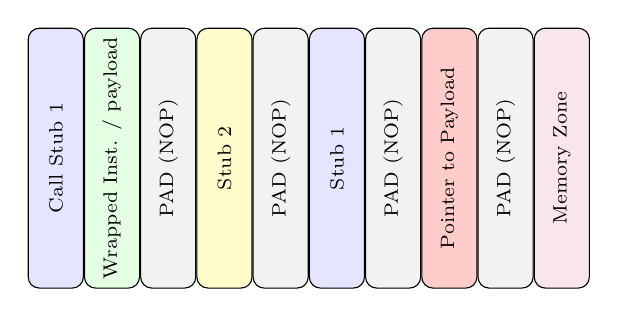
\begin{tikzpicture}[
    font=\scriptsize,
    node distance=0.0cm,
    every node/.style={
        rotate=90,
        minimum width=3.3cm,
        minimum height=0.7cm,
        text centered,
        draw,
        fill=gray!10,
        rounded corners,
        inner xsep=2pt,
        inner ysep=6pt
    }
]

\node (stubCall)  [fill=blue!10]    {Call Stub 1};
\node (payload)   [below=of stubCall, fill=green!10]  {Wrapped Inst. / payload};
\node (pad1)      [below=of payload]                  {PAD (NOP)};
\node (stub2)     [below=of pad1, fill=yellow!20]     {Stub 2};
\node (pad2)      [below=of stub2]                    {PAD (NOP)};
\node (stub1)     [below=of pad2, fill=blue!10]       {Stub 1};
\node (pad3)      [below=of stub1]                    {PAD (NOP)};
\node (payloadPtr)[below=of pad3, fill=red!20]        {Pointer to Payload};
\node (pad4)      [below=of payloadPtr]               {PAD (NOP)};
\node (memZone)   [below=of pad4, fill=purple!10]     {Memory Zone};

\end{tikzpicture}
\Description{A schematic separates the initial call, instruction wrappers, redirector components, padding, offset information, and memory region.}
\caption{PII payload layout. Adapted from Fig.~1 of~\cite{zone_secrypt_2026}.}
\label{fig:pii_layout}
\end{figure}

The representation consists of four components:

\begin{enumerate}
  \item \textbf{Base-Address Stub (Stub1).}
This component determines the runtime base address and records it in a designated memory location.

  \item \textbf{Redirector Stub (Stub2).}
This component obtains the next logical instruction location from the offset table and dispatches execution to it.

  \item \textbf{Offset Table.}
This contiguous table contains the instruction offsets used by the redirector.

  \item \textbf{Wrapped Instructions.}
Each input instruction is placed in a wrapper intended to maintain the required register, flag, and stack state.
\end{enumerate}

\paragraph{Execution Sequence.}
The conference paper describes execution in three phases:
\begin{itemize}
    \item \textbf{Initialization.} A call enters Stub1 (Listing~\ref{lst:stub1}). The return address supplied by that call is used to establish the payload's runtime location.
    \item \textbf{Original operation.} The wrapper in Listing~\ref{lst:instrWrap} restores the saved state, adjusts the stack, executes the input instruction, and supplies its logical index to Stub2.
    \item \textbf{Dispatch.} The redirector in Listing~\ref{lst:stub2red} saves the state it uses, obtains the successor's location from the offset table and base address, and transfers control to that wrapper after restoring the relevant state.

\end{itemize}

\paragraph{Physical Placement.}
The original implementation permutes complete wrappers, treating each five-instruction wrapper as a unit. The offset table is updated for the resulting placement. Execution still starts with the initial call to Stub1; logical succession is represented by the table rather than by the wrappers' physical adjacency.

\begin{lstlisting}[label={lst:stub1},language={[x86masm]Assembler}, basicstyle=\scriptsize\ttfamily, caption={Base-address component. Reproduced from Listing~1 of~\cite{zone_secrypt_2026}.}]
pop <random_unused_reg>;    popping 2nd instruction address
mov [<random_unused_reg> - 5 + <init_address>],  <random_unused_reg>; move it to a memory slot
push <random_unused_reg>; push just to avoid altering the stack
jmp <random_unused_reg>; return to the caller (2nd instruction)
\end{lstlisting}

\begin{lstlisting}[label={lst:instrWrap}, language={[x86masm]Assembler}, basicstyle=\scriptsize\ttfamily, caption={Instruction wrapper. Reproduced from Listing~2 of~\cite{zone_secrypt_2026}.}]
pop rax;                    ; popping rax because we just used it to save jmp address
lea rsp, [rsp + 8];         ; adjusting stack to avoid stack overflow
ORIGINAL_INSTRUCTION;       ; original instruction
push <0x3e8 + counter>;     ; pushing instruction original index + a constant
jmp <stub2_address>;        ; Jumping to 'redirector' stub 
\end{lstlisting}

\begin{lstlisting}[label={lst:stub2red},language={[x86masm]Assembler}, basicstyle=\scriptsize\ttfamily, caption={x64 redirector. Reproduced from Listing~3 of~\cite{zone_secrypt_2026}.}]
push rax;                                       saving original 'rax' register state
push rcx;                                       saving original 'rcx' register state
mov rcx, [rsp + 0x10] ;                         getting the instruction index from the stack.
pushf;                                          saving original CPU flags
sub rcx, 0x3e8; ;                               subtracting a constant to get instr index
inc rcx;                                        increase instruction number
mov rax, [rip + init_addr_offset];              get payload base address
mov rcx, [rax + mem_address - 5 + rcx * 8];     get next instruction address
sub rcx, 0x5;                                   just because base address is 2nd instruction
add rax, rcx;                                   add payload base address to the offset
popf;                                           restore cpu flags
pop rcx;                                        restore rcx value
jmp rax;                                        jmp to next instruction
\end{lstlisting}

\paragraph{Architectural Variants.}
Listings~\ref{lst:stub2red} and~\ref{lst:stub286} show the published x64 and x86 redirectors. In addition to the different register widths, they differ in how the required address is obtained: the x86 version uses the call-based mechanism documented in the original listing rather than x64 RIP-relative addressing.

\begin{lstlisting}[label={lst:stub286},language={[x86masm]Assembler}, basicstyle=\scriptsize\ttfamily, caption={x86 redirector. Reproduced from Listing~4 of~\cite{zone_secrypt_2026}.}]
push eax;
push ecx;
mov ecx, [esp + 0x8]
pushf;
sub ecx, 0x3e8;
inc ecx;

call <stub2_address + 0x14>;    calling pop eax, 0x14 is pop eax offset from stub2 address
pop eax;                        popping eax puts in eax the value of the instruction pointer

mov eax, [eax + <init_addr_offset>];
mov ecx, [eax + <mem_address> - 5 + ecx * 4];
sub ecx, 0x5
add eax, ecx
popf;
pop ecx;
jmp eax;
\end{lstlisting}

\subsection{How Instructions Are Patched}\label{sec:instr_patch}

Moving instructions or inserting bytes can invalidate references to their previous locations. The patching phase updates control-flow destinations and other affected references to the modified layout. Branches and calls are therefore part of the rewriting process, not merely instructions that can be copied without regard to their new positions.

This requirement also explains the scope restriction. Rewriting raw instruction sequences already requires consistent target updates; complete PE files introduce additional metadata and layout dependencies. Algorithm~\ref{alg:zonealg} reproduces the high-level workflow from~\cite{zone_secrypt_2026}.

\begin{algorithm}[t]

\caption{High-level Zone workflow. Reproduced from Algorithm~1 of~\cite{zone_secrypt_2026}.}\label{alg:zonealg}

\scriptsize

\SetKwProg{Fn}{Function}{}{}
\SetKwFor{ForEach}{for each}{}{end}
\SetKwIF{If}{ElseIf}{Else}{if}{}{else if}{else}{end}

\KwData{raw\_bytes}
\KwResult{Transformed binary}

\textbf{global} instruction\_list $\gets$ []\;
\textbf{global} instruction\_dict $\gets$ \{\}\;
\textbf{global} label\_table $\gets$ []\;

\BlankLine

\Fn{\textbf{disass} \label{fun:disas} }{

    CAPSTONE.SKIPDATA $\gets$ TRUE\;\label{fun:skipdata}

    \ForEach{instruction in disasm(raw\_bytes)}{
        instruction\_list.append(instruction)\;
        instruction\_dict[instruction.address] $\gets$ instruction\;

        \If{instruction is X86.Control\_flow\_instruction}{
            jump\_address $\gets$ extract\_address(instruction.op\_string)\;
            label\_table.append((instruction, instruction\_dict[jump\_address]))\;
        }
    }
}

\BlankLine

\Fn{\textbf{update\_instructions} \label{fun:update_instr}}{
    new\_instruction\_dict $\gets$ \{\}\;

    \ForEach{instruction in instruction\_list}{
        address $\gets$ instruction.previous\_instruction.address + len(instruction.previous\_instruction.bytes)\;
        instruction.address $\gets$ address\;

        new\_instruction\_dict[instruction.address] $\gets$ instruction\;
    }

    instruction\_dict $\gets$ new\_instruction\_dict\;
}

\BlankLine

\Fn{\textbf{morph} \label{fun:morph}} {
    equal\_code\_substitution()\;
    nop\_insertion()\;
    instruction\_block\_shuffling()\;
    bogus\_control\_flow()\;
    position\_independent\_instruction()\;
}

\BlankLine

\Fn{\textbf{adjust\_label\_table} \label{fun:adj_lab_tab}}{
    update\_instructions()\;

    \ForEach{entry in label\_table}{
        jmp\_addr $\gets$ extract\_address(entry[0].op\_string)\;
        jmp\_addr\_new $\gets$ entry[1].address\;

        new\_instruction $\gets$ keystone.assemble(
        ``entry[0].mnemonic jmp\_addr\_new'')\;

        entry[0] $\gets$ new\_instruction\;
    }
}

\BlankLine

\Fn{\textbf{main}}{
    disass()\;
    morph()\;
    adjust\_label\_table()\;
    write\_to\_file()\; \label{fun:writefile}
}

\end{algorithm}

\subsection{Transformation Pipeline}
The original workflow in Algorithm~\ref{alg:zonealg} can be read as six stages. The additional analysis and transformation paths are described in Sections~\ref{sec:code_data}--\ref{sec:wrapping}.

\begin{enumerate}
\item \textbf{Input representation.}
    Capstone produces instruction objects held in a linked sequence, with an address-indexed dictionary for lookup (Line~\ref{fun:disas}).

\item \textbf{Embedded data.}
    The implementation enables Capstone's \texttt{Skipdata} option (Line~\ref{fun:skipdata}). This does not solve the general problem of identifying inline data, particularly when data bytes also admit an instruction interpretation~\cite{bin2binobf}.

\item \textbf{Reference tracking.}
    A label table associates each tracked control-flow operation with its target instruction object. This association is retained as the object's physical address changes.

\item \textbf{Transformation and layout update.}
    The chosen transformations are applied (Line~\ref{fun:morph}), followed by recomputation of instruction addresses (Line~\ref{fun:update_instr}).

\item \textbf{Reassembly of tracked branches.}
    Keystone assembles the tracked control-flow operations using their updated targets (Line~\ref{fun:adj_lab_tab}).

\item \textbf{Output.}
    The resulting instruction bytes are written as a new raw binary (Line~\ref{fun:writefile}).

\end{enumerate}

\section{Published Experimental Baseline}\label{sec:results}
\draftnote{The detailed historical plots and their reported numerical
values are retained from the preparation manuscript. Some category/value
associations in the detection and working-rate plots, and the provenance
of the similarity metric, require reconciliation against the conference
version and archived records. These are baseline editorial checks,
not replacement experiments. See \texttt{BASELINE\_CHECKS.md}.}

This section restates the protocol and results of the conference paper~\cite{zone_secrypt_2026}. It introduces no additional measurements. VirusTotal scans supplied verdicts from more than 70 engines, subject to the file-format limitations discussed below.

The corpus contains 102 Windows payloads: 38 x64 inputs and 64 x86 inputs. Most originate from the Metasploit Framework and include reverse and bind shells. This provides an identifiable collection of payload types, but does not constitute a representative sample of all Windows malware.

Two scope restrictions are relevant to interpretation:
\begin{itemize}
    \item \textbf{Architecture coverage.} The x64 and x86 sets differ in size and membership. Architecture-level comparisons therefore also reflect differences between the two input collections.
    \item \textbf{Excluded inputs.} Large, DLL-based command-and-control components are outside the payload-level scope. Their PE structure and embedded data introduce additional rewriting dependencies.

\end{itemize}

\paragraph{Testing Method.}
Each of the fifteen configurations was applied to every input, with ten generated variants per input and configuration to expose variation in the transformation process. The five individual transformations and ten combinations were:

\begin{itemize}
    \item \textbf{Single:} NOP (\texttt{nop}), Equal Code Substitution (\texttt{eq}), Bogus Control Flow (\texttt{bcf}), Instruction Block Permutation (\texttt{ibp}), and Position-Independent Instruction (\texttt{pii}).
    \item \textbf{Combined:} \texttt{eq\_nop\_bcf}, \texttt{eq\_nop\_ibp}, \texttt{eq\_nop\_pii}, \texttt{eq\_nop}, \texttt{eq\_bcf}, \texttt{eq\_ibp}, \texttt{eq\_pii}, \texttt{nop\_bcf}, \texttt{nop\_ibp} and \texttt{nop\_pii}.
\end{itemize}

The \emph{detection rate} for an individual file is the fraction of scanning engines that returned a malicious verdict; summaries aggregate these per-file measurements. Figure~\ref{fig:all_payloads} presents the published transformed-file results. The corresponding baseline averages for the original files were 21.67\% for x64 and 22.63\% for x86.

\begin{figure}[tbp]
\centering
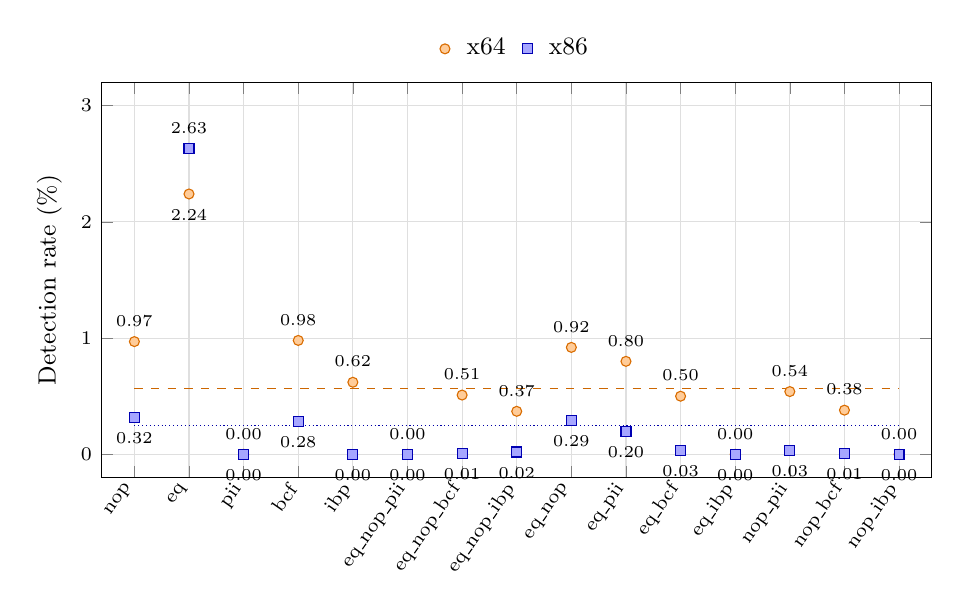
\begin{tikzpicture}
\begin{axis}[
width=\linewidth,height=6.6cm,
ylabel={Detection rate (\%)},ymin=-0.2,ymax=3.2,xmin=-0.6,xmax=14.6,
xtick={0,...,14},
xticklabels={nop,eq,pii,bcf,ibp,eq\_nop\_pii,eq\_nop\_bcf,eq\_nop\_ibp,eq\_nop,eq\_pii,eq\_bcf,eq\_ibp,nop\_pii,nop\_bcf,nop\_ibp},
xticklabel style={rotate=55,anchor=east,font=\scriptsize},
yticklabel style={font=\scriptsize},label style={font=\small},
grid=major,grid style={gray!25},scaled y ticks=false,
legend style={at={(0.5,1.03)},anchor=south,legend columns=2,column sep=4pt,font=\small,draw=none},
clip=false,
]
\addplot[orange!80!black,dashed,no marks,forget plot] coordinates {(0,0.57) (14,0.57)};
\addplot[blue!65!black,densely dotted,no marks,forget plot] coordinates {(0,0.25) (14,0.25)};
\addplot[only marks,mark size=1.8pt,orange!85!black,mark=*,mark options={fill=orange!40}] coordinates {(0,0.97) (1,2.24) (2,0.00) (3,0.98) (4,0.62) (5,0.00) (6,0.51) (7,0.37) (8,0.92) (9,0.80) (10,0.50) (11,0.00) (12,0.54) (13,0.38) (14,0.00)};
\addlegendentry{x64}
\node[anchor=south,yshift=2pt,font=\fontsize{6}{7}\selectfont] at (axis cs:0,0.97) {0.97};
\node[anchor=north,yshift=-2pt,font=\fontsize{6}{7}\selectfont] at (axis cs:1,2.24) {2.24};
\node[anchor=south,yshift=2pt,font=\fontsize{6}{7}\selectfont] at (axis cs:2,0.00) {0.00};
\node[anchor=south,yshift=2pt,font=\fontsize{6}{7}\selectfont] at (axis cs:3,0.98) {0.98};
\node[anchor=south,yshift=2pt,font=\fontsize{6}{7}\selectfont] at (axis cs:4,0.62) {0.62};
\node[anchor=south,yshift=2pt,font=\fontsize{6}{7}\selectfont] at (axis cs:5,0.00) {0.00};
\node[anchor=south,yshift=2pt,font=\fontsize{6}{7}\selectfont] at (axis cs:6,0.51) {0.51};
\node[anchor=south,yshift=2pt,font=\fontsize{6}{7}\selectfont] at (axis cs:7,0.37) {0.37};
\node[anchor=south,yshift=2pt,font=\fontsize{6}{7}\selectfont] at (axis cs:8,0.92) {0.92};
\node[anchor=south,yshift=2pt,font=\fontsize{6}{7}\selectfont] at (axis cs:9,0.80) {0.80};
\node[anchor=south,yshift=2pt,font=\fontsize{6}{7}\selectfont] at (axis cs:10,0.50) {0.50};
\node[anchor=south,yshift=2pt,font=\fontsize{6}{7}\selectfont] at (axis cs:11,0.00) {0.00};
\node[anchor=south,yshift=2pt,font=\fontsize{6}{7}\selectfont] at (axis cs:12,0.54) {0.54};
\node[anchor=south,yshift=2pt,font=\fontsize{6}{7}\selectfont] at (axis cs:13,0.38) {0.38};
\node[anchor=south,yshift=2pt,font=\fontsize{6}{7}\selectfont] at (axis cs:14,0.00) {0.00};
\addplot[only marks,mark size=1.8pt,blue!70!black,mark=square*,mark options={fill=blue!35}] coordinates {(0,0.32) (1,2.63) (2,0.00) (3,0.28) (4,0.00) (5,0.00) (6,0.01) (7,0.02) (8,0.29) (9,0.20) (10,0.03) (11,0.00) (12,0.03) (13,0.01) (14,0.00)};
\addlegendentry{x86}
\node[anchor=north,yshift=-2pt,font=\fontsize{6}{7}\selectfont] at (axis cs:0,0.32) {0.32};
\node[anchor=south,yshift=2pt,font=\fontsize{6}{7}\selectfont] at (axis cs:1,2.63) {2.63};
\node[anchor=north,yshift=-2pt,font=\fontsize{6}{7}\selectfont] at (axis cs:2,0.00) {0.00};
\node[anchor=north,yshift=-2pt,font=\fontsize{6}{7}\selectfont] at (axis cs:3,0.28) {0.28};
\node[anchor=north,yshift=-2pt,font=\fontsize{6}{7}\selectfont] at (axis cs:4,0.00) {0.00};
\node[anchor=north,yshift=-2pt,font=\fontsize{6}{7}\selectfont] at (axis cs:5,0.00) {0.00};
\node[anchor=north,yshift=-2pt,font=\fontsize{6}{7}\selectfont] at (axis cs:6,0.01) {0.01};
\node[anchor=north,yshift=-2pt,font=\fontsize{6}{7}\selectfont] at (axis cs:7,0.02) {0.02};
\node[anchor=north,yshift=-2pt,font=\fontsize{6}{7}\selectfont] at (axis cs:8,0.29) {0.29};
\node[anchor=north,yshift=-2pt,font=\fontsize{6}{7}\selectfont] at (axis cs:9,0.20) {0.20};
\node[anchor=north,yshift=-2pt,font=\fontsize{6}{7}\selectfont] at (axis cs:10,0.03) {0.03};
\node[anchor=north,yshift=-2pt,font=\fontsize{6}{7}\selectfont] at (axis cs:11,0.00) {0.00};
\node[anchor=north,yshift=-2pt,font=\fontsize{6}{7}\selectfont] at (axis cs:12,0.03) {0.03};
\node[anchor=north,yshift=-2pt,font=\fontsize{6}{7}\selectfont] at (axis cs:13,0.01) {0.01};
\node[anchor=north,yshift=-2pt,font=\fontsize{6}{7}\selectfont] at (axis cs:14,0.00) {0.00};
\end{axis}
\end{tikzpicture}
\Description{Malicious-verdict fractions in raw-file scans. Dashed reference lines show the reported architecture averages (x64: 0.57\%; x86: 0.25\%). Orange circles identify x64 and blue squares identify x86.}
\caption{Malicious-verdict fractions in raw-file scans. Dashed reference lines show the reported architecture averages (x64: 0.57\%; x86: 0.25\%). Data from Fig.~2 of~\cite{zone_secrypt_2026}; redrawn for the present format.}
\label{fig:all_payloads}
\end{figure}

The plotted observations vary by transformation and architecture. Several configurations involving PII received no malicious verdicts in these raw-file scans, whereas EQ retained more detections. These measurements describe the tested representations and submission conditions; they should be interpreted together with the functional results.

\label{par:working_rate}
The \emph{working rate} is the proportion of variants that passed the original execution checks (Figure~\ref{fig:working_rate}). Those checks observed the expected connection for reverse shells, port opening for bind shells, and exception-free termination for the remaining generic cases. The tests are empirical functional checks rather than proofs of semantic equivalence. The conference paper reported greater overall stability for EQ and lower stability for PII, particularly in the x86 collection; the results also varied substantially across combined configurations.

\begin{figure}[tbp]
\centering
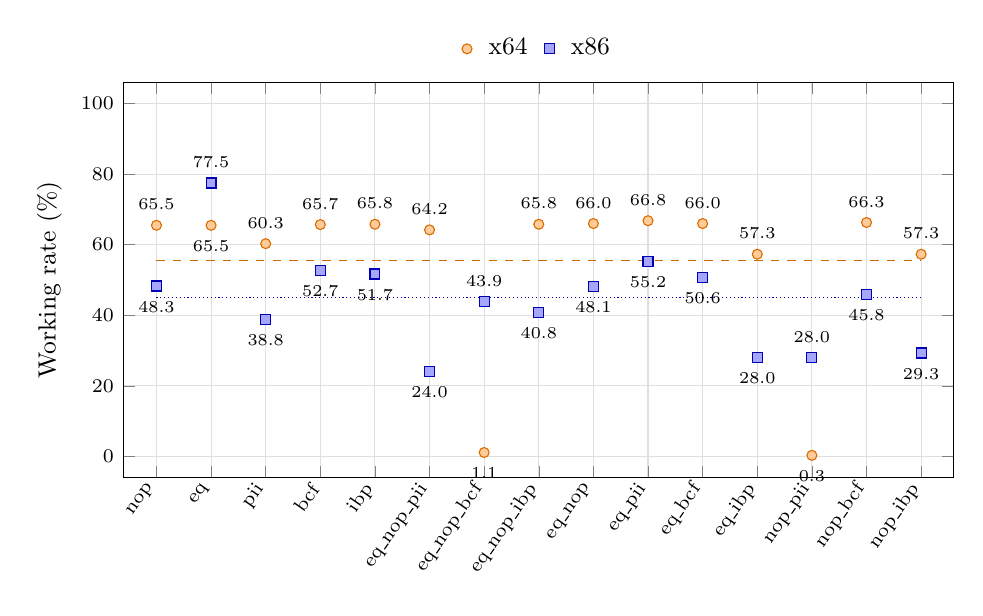
\begin{tikzpicture}
\begin{axis}[
width=\linewidth,height=6.6cm,
ylabel={Working rate (\%)},ymin=-6,ymax=106,xmin=-0.6,xmax=14.6,
xtick={0,...,14},
xticklabels={nop,eq,pii,bcf,ibp,eq\_nop\_pii,eq\_nop\_bcf,eq\_nop\_ibp,eq\_nop,eq\_pii,eq\_bcf,eq\_ibp,nop\_pii,nop\_bcf,nop\_ibp},
xticklabel style={rotate=55,anchor=east,font=\scriptsize},
yticklabel style={font=\scriptsize},label style={font=\small},
grid=major,grid style={gray!25},scaled y ticks=false,
legend style={at={(0.5,1.03)},anchor=south,legend columns=2,column sep=4pt,font=\small,draw=none},
clip=false,
]
\addplot[orange!80!black,dashed,no marks,forget plot] coordinates {(0,55.6) (14,55.6)};
\addplot[blue!65!black,densely dotted,no marks,forget plot] coordinates {(0,45.0) (14,45.0)};
\addplot[only marks,mark size=1.8pt,orange!85!black,mark=*,mark options={fill=orange!40}] coordinates {(0,65.5) (1,65.5) (2,60.3) (3,65.7) (4,65.8) (5,64.2) (6,1.1) (7,65.8) (8,66.0) (9,66.8) (10,66.0) (11,57.3) (12,0.3) (13,66.3) (14,57.3)};
\addlegendentry{x64}
\node[anchor=south,yshift=2pt,font=\fontsize{6}{7}\selectfont] at (axis cs:0,65.5) {65.5};
\node[anchor=north,yshift=-2pt,font=\fontsize{6}{7}\selectfont] at (axis cs:1,65.5) {65.5};
\node[anchor=south,yshift=2pt,font=\fontsize{6}{7}\selectfont] at (axis cs:2,60.3) {60.3};
\node[anchor=south,yshift=2pt,font=\fontsize{6}{7}\selectfont] at (axis cs:3,65.7) {65.7};
\node[anchor=south,yshift=2pt,font=\fontsize{6}{7}\selectfont] at (axis cs:4,65.8) {65.8};
\node[anchor=south,yshift=2pt,font=\fontsize{6}{7}\selectfont] at (axis cs:5,64.2) {64.2};
\node[anchor=north,yshift=-2pt,font=\fontsize{6}{7}\selectfont] at (axis cs:6,1.1) {1.1};
\node[anchor=south,yshift=2pt,font=\fontsize{6}{7}\selectfont] at (axis cs:7,65.8) {65.8};
\node[anchor=south,yshift=2pt,font=\fontsize{6}{7}\selectfont] at (axis cs:8,66.0) {66.0};
\node[anchor=south,yshift=2pt,font=\fontsize{6}{7}\selectfont] at (axis cs:9,66.8) {66.8};
\node[anchor=south,yshift=2pt,font=\fontsize{6}{7}\selectfont] at (axis cs:10,66.0) {66.0};
\node[anchor=south,yshift=2pt,font=\fontsize{6}{7}\selectfont] at (axis cs:11,57.3) {57.3};
\node[anchor=north,yshift=-2pt,font=\fontsize{6}{7}\selectfont] at (axis cs:12,0.3) {0.3};
\node[anchor=south,yshift=2pt,font=\fontsize{6}{7}\selectfont] at (axis cs:13,66.3) {66.3};
\node[anchor=south,yshift=2pt,font=\fontsize{6}{7}\selectfont] at (axis cs:14,57.3) {57.3};
\addplot[only marks,mark size=1.8pt,blue!70!black,mark=square*,mark options={fill=blue!35}] coordinates {(0,48.3) (1,77.5) (2,38.8) (3,52.7) (4,51.7) (5,24.0) (6,43.9) (7,40.8) (8,48.1) (9,55.2) (10,50.6) (11,28.0) (12,28.0) (13,45.8) (14,29.3)};
\addlegendentry{x86}
\node[anchor=north,yshift=-2pt,font=\fontsize{6}{7}\selectfont] at (axis cs:0,48.3) {48.3};
\node[anchor=south,yshift=2pt,font=\fontsize{6}{7}\selectfont] at (axis cs:1,77.5) {77.5};
\node[anchor=north,yshift=-2pt,font=\fontsize{6}{7}\selectfont] at (axis cs:2,38.8) {38.8};
\node[anchor=north,yshift=-2pt,font=\fontsize{6}{7}\selectfont] at (axis cs:3,52.7) {52.7};
\node[anchor=north,yshift=-2pt,font=\fontsize{6}{7}\selectfont] at (axis cs:4,51.7) {51.7};
\node[anchor=north,yshift=-2pt,font=\fontsize{6}{7}\selectfont] at (axis cs:5,24.0) {24.0};
\node[anchor=south,yshift=2pt,font=\fontsize{6}{7}\selectfont] at (axis cs:6,43.9) {43.9};
\node[anchor=north,yshift=-2pt,font=\fontsize{6}{7}\selectfont] at (axis cs:7,40.8) {40.8};
\node[anchor=north,yshift=-2pt,font=\fontsize{6}{7}\selectfont] at (axis cs:8,48.1) {48.1};
\node[anchor=north,yshift=-2pt,font=\fontsize{6}{7}\selectfont] at (axis cs:9,55.2) {55.2};
\node[anchor=north,yshift=-2pt,font=\fontsize{6}{7}\selectfont] at (axis cs:10,50.6) {50.6};
\node[anchor=north,yshift=-2pt,font=\fontsize{6}{7}\selectfont] at (axis cs:11,28.0) {28.0};
\node[anchor=south,yshift=2pt,font=\fontsize{6}{7}\selectfont] at (axis cs:12,28.0) {28.0};
\node[anchor=north,yshift=-2pt,font=\fontsize{6}{7}\selectfont] at (axis cs:13,45.8) {45.8};
\node[anchor=north,yshift=-2pt,font=\fontsize{6}{7}\selectfont] at (axis cs:14,29.3) {29.3};
\end{axis}
\end{tikzpicture}
\Description{Variants passing the published functional checks. Dashed reference lines show the reported architecture averages (x64: 55.6\%; x86: 45.0\%). Orange circles identify x64 and blue squares identify x86.}
\caption{Variants passing the published functional checks. Dashed reference lines show the reported architecture averages (x64: 55.6\%; x86: 45.0\%). Data from Fig.~3 of~\cite{zone_secrypt_2026}; redrawn for the present format.}
\label{fig:working_rate}
\end{figure}

\paragraph{Evaluation Limitations.}
A raw \texttt{.bin} submission is not a complete executable application. Engines may apply a different analysis path to such input, omit execution-based analysis, or decline to analyze an unsupported representation. Low detection fractions therefore cannot be interpreted as an evaluation of complete antivirus or endpoint detection and response (EDR) products during deployment.

Submitting original and transformed payloads under the same format assumptions provides a limited basis for comparing the representations in this corpus. It does not remove format-dependent biases or establish behavior under other execution conditions. The published results should be read within those boundaries~\cite{zone_secrypt_2026}.
% Extended assessment follows the original results and SGN comparison.

\section{Size and Statistical Measurements}\label{sect:var_metrics}
The conference paper also characterized how the transformed representations differ from their inputs~\cite{zone_secrypt_2026}. Its three additional measurements were:

\begin{itemize}
    \item Payload length variation.
    \item Delta entropy.
    \item Cosine similarity.
\end{itemize}

\paragraph{Payload Length Variation.}
Let $L_i$ denote the byte length of a transformed file and let $n$ be the number of files considered for a configuration. The reported mean length is:
\[
\overline{L} = \frac{1}{n} \sum_{i=1}^{n} L_i
\]

\begin{figure}[tbp]
\centering
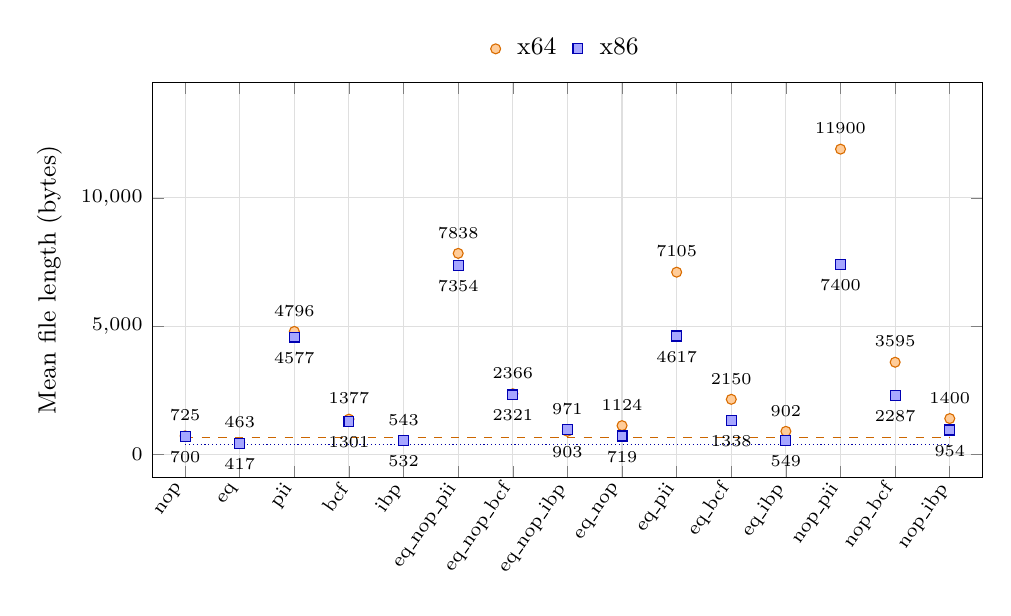
\begin{tikzpicture}
\begin{axis}[
width=\linewidth,height=6.6cm,
ylabel={Mean file length (bytes)},ymin=-900,ymax=14500,xmin=-0.6,xmax=14.6,
xtick={0,...,14},
xticklabels={nop,eq,pii,bcf,ibp,eq\_nop\_pii,eq\_nop\_bcf,eq\_nop\_ibp,eq\_nop,eq\_pii,eq\_bcf,eq\_ibp,nop\_pii,nop\_bcf,nop\_ibp},
xticklabel style={rotate=55,anchor=east,font=\scriptsize},
yticklabel style={font=\scriptsize},label style={font=\small},
grid=major,grid style={gray!25},scaled y ticks=false,
legend style={at={(0.5,1.03)},anchor=south,legend columns=2,column sep=4pt,font=\small,draw=none},
clip=false,
]
\addplot[orange!80!black,dashed,no marks,forget plot] coordinates {(0,652.632) (14,652.632)};
\addplot[blue!65!black,densely dotted,no marks,forget plot] coordinates {(0,400.750) (14,400.750)};
\addplot[only marks,mark size=1.8pt,orange!85!black,mark=*,mark options={fill=orange!40}] coordinates {(0,725) (1,463) (2,4796) (3,1377) (4,543) (5,7838) (6,2366) (7,903) (8,1124) (9,7105) (10,2150) (11,902) (12,11900) (13,3595) (14,1400)};
\addlegendentry{x64}
\node[anchor=south,yshift=2pt,font=\fontsize{6}{7}\selectfont] at (axis cs:0,725) {725};
\node[anchor=south,yshift=2pt,font=\fontsize{6}{7}\selectfont] at (axis cs:1,463) {463};
\node[anchor=south,yshift=2pt,font=\fontsize{6}{7}\selectfont] at (axis cs:2,4796) {4796};
\node[anchor=south,yshift=2pt,font=\fontsize{6}{7}\selectfont] at (axis cs:3,1377) {1377};
\node[anchor=south,yshift=2pt,font=\fontsize{6}{7}\selectfont] at (axis cs:4,543) {543};
\node[anchor=south,yshift=2pt,font=\fontsize{6}{7}\selectfont] at (axis cs:5,7838) {7838};
\node[anchor=south,yshift=2pt,font=\fontsize{6}{7}\selectfont] at (axis cs:6,2366) {2366};
\node[anchor=north,yshift=-2pt,font=\fontsize{6}{7}\selectfont] at (axis cs:7,903) {903};
\node[anchor=south,yshift=2pt,font=\fontsize{6}{7}\selectfont] at (axis cs:8,1124) {1124};
\node[anchor=south,yshift=2pt,font=\fontsize{6}{7}\selectfont] at (axis cs:9,7105) {7105};
\node[anchor=south,yshift=2pt,font=\fontsize{6}{7}\selectfont] at (axis cs:10,2150) {2150};
\node[anchor=south,yshift=2pt,font=\fontsize{6}{7}\selectfont] at (axis cs:11,902) {902};
\node[anchor=south,yshift=2pt,font=\fontsize{6}{7}\selectfont] at (axis cs:12,11900) {11900};
\node[anchor=south,yshift=2pt,font=\fontsize{6}{7}\selectfont] at (axis cs:13,3595) {3595};
\node[anchor=south,yshift=2pt,font=\fontsize{6}{7}\selectfont] at (axis cs:14,1400) {1400};
\addplot[only marks,mark size=1.8pt,blue!70!black,mark=square*,mark options={fill=blue!35}] coordinates {(0,700) (1,417) (2,4577) (3,1301) (4,532) (5,7354) (6,2321) (7,971) (8,719) (9,4617) (10,1338) (11,549) (12,7400) (13,2287) (14,954)};
\addlegendentry{x86}
\node[anchor=north,yshift=-2pt,font=\fontsize{6}{7}\selectfont] at (axis cs:0,700) {700};
\node[anchor=north,yshift=-2pt,font=\fontsize{6}{7}\selectfont] at (axis cs:1,417) {417};
\node[anchor=north,yshift=-2pt,font=\fontsize{6}{7}\selectfont] at (axis cs:2,4577) {4577};
\node[anchor=north,yshift=-2pt,font=\fontsize{6}{7}\selectfont] at (axis cs:3,1301) {1301};
\node[anchor=north,yshift=-2pt,font=\fontsize{6}{7}\selectfont] at (axis cs:4,532) {532};
\node[anchor=north,yshift=-2pt,font=\fontsize{6}{7}\selectfont] at (axis cs:5,7354) {7354};
\node[anchor=north,yshift=-2pt,font=\fontsize{6}{7}\selectfont] at (axis cs:6,2321) {2321};
\node[anchor=south,yshift=2pt,font=\fontsize{6}{7}\selectfont] at (axis cs:7,971) {971};
\node[anchor=north,yshift=-2pt,font=\fontsize{6}{7}\selectfont] at (axis cs:8,719) {719};
\node[anchor=north,yshift=-2pt,font=\fontsize{6}{7}\selectfont] at (axis cs:9,4617) {4617};
\node[anchor=north,yshift=-2pt,font=\fontsize{6}{7}\selectfont] at (axis cs:10,1338) {1338};
\node[anchor=north,yshift=-2pt,font=\fontsize{6}{7}\selectfont] at (axis cs:11,549) {549};
\node[anchor=north,yshift=-2pt,font=\fontsize{6}{7}\selectfont] at (axis cs:12,7400) {7400};
\node[anchor=north,yshift=-2pt,font=\fontsize{6}{7}\selectfont] at (axis cs:13,2287) {2287};
\node[anchor=north,yshift=-2pt,font=\fontsize{6}{7}\selectfont] at (axis cs:14,954) {954};
\end{axis}
\end{tikzpicture}
\Description{Mean transformed-file length. Reference lines indicate the original-file means (x64: 652.632 bytes; x86: 400.750 bytes). Orange circles identify x64 and blue squares identify x86.}
\caption{Mean transformed-file length. Reference lines indicate the original-file means (x64: 652.632 bytes; x86: 400.750 bytes). Data from Fig.~4 of~\cite{zone_secrypt_2026}; redrawn for the present format.}
\label{fig:length_comparison}
\end{figure}

The size results in Figure~\ref{fig:length_comparison} show substantial growth for PII and BCF configurations. Some EQ-containing configurations instead produced smaller average outputs than the original-file reference. The conference paper associated this observation with the implementation's treatment of data during disassembly; the size measurement alone does not establish that any removed bytes were semantically irrelevant.

\paragraph{Delta Entropy.}
The reported entropy change compares the transformed representation, $H_{tech}$, with its original, $H_{orig}$, using the percentage difference:

\begin{equation}
\Delta H \; (\%) = \frac{H_{tech} - H_{orig}}{H_{orig}} \times 100
\end{equation}

The measurements were computed on raw bytes and on tokenized assembly. Figures~\ref{fig:shan_entropy} and~\ref{fig:shan_entropy_bytes} retain the published results. The assembly-based representation also permits comparison with the metrics discussed by Mohseni et al.~\cite{llmobf}.

In the assembly results, NOP insertion increased entropy for both architectures, while PII decreased it. The latter observation is consistent with the repeated bookkeeping instructions in the wrapper representation. A small entropy change does not, by itself, imply a small change in control-flow organization. The conference paper illustrated this limitation using BCF and IBP:

\begin{itemize}
\item \textbf{BCF.} A small entropy difference coexisted with greater length and a changed opcode distribution (Figure~\ref{fig:cosine_similarity}).
    \item \textbf{IBP.} Moving blocks can change their layout while retaining much of their instruction-frequency distribution.

\end{itemize}

Entropy is consequently treated as a descriptive statistic of the chosen representation, not a standalone measure of structural complexity or functional preservation.

\begin{figure}[tbp]
\centering
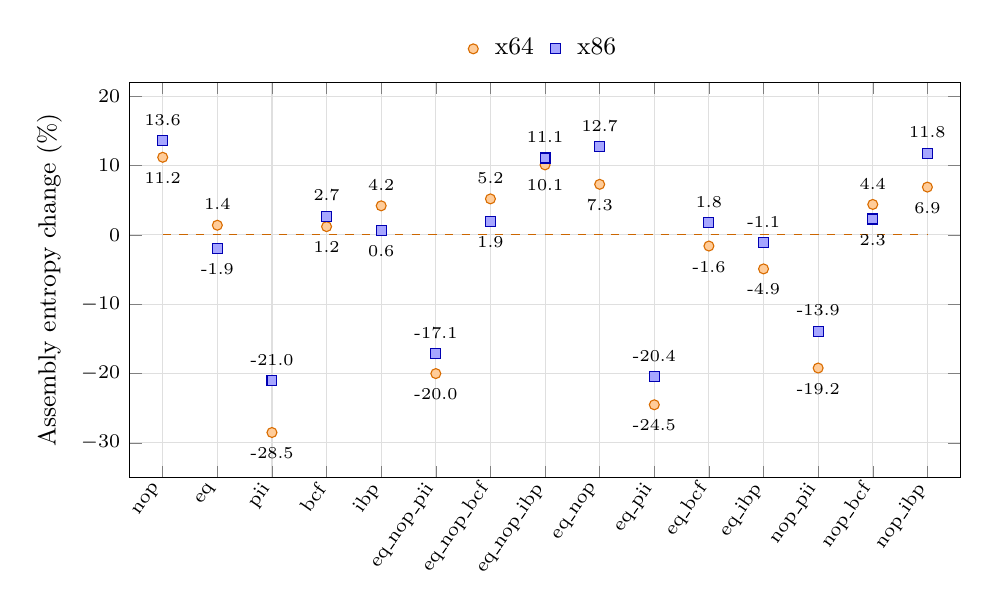
\begin{tikzpicture}
\begin{axis}[
width=\linewidth,height=6.6cm,
ylabel={Assembly entropy change (\%)},ymin=-35,ymax=22,xmin=-0.6,xmax=14.6,
xtick={0,...,14},
xticklabels={nop,eq,pii,bcf,ibp,eq\_nop\_pii,eq\_nop\_bcf,eq\_nop\_ibp,eq\_nop,eq\_pii,eq\_bcf,eq\_ibp,nop\_pii,nop\_bcf,nop\_ibp},
xticklabel style={rotate=55,anchor=east,font=\scriptsize},
yticklabel style={font=\scriptsize},label style={font=\small},
grid=major,grid style={gray!25},scaled y ticks=false,
legend style={at={(0.5,1.03)},anchor=south,legend columns=2,column sep=4pt,font=\small,draw=none},
clip=false,
]
\addplot[orange!80!black,dashed,no marks,forget plot] coordinates {(0,0) (14,0)};
\addplot[only marks,mark size=1.8pt,orange!85!black,mark=*,mark options={fill=orange!40}] coordinates {(0,11.2) (1,1.4) (2,-28.5) (3,1.2) (4,4.2) (5,-20.0) (6,5.2) (7,10.1) (8,7.3) (9,-24.5) (10,-1.6) (11,-4.9) (12,-19.2) (13,4.4) (14,6.9)};
\addlegendentry{x64}
\node[anchor=north,yshift=-2pt,font=\fontsize{6}{7}\selectfont] at (axis cs:0,11.2) {11.2};
\node[anchor=south,yshift=2pt,font=\fontsize{6}{7}\selectfont] at (axis cs:1,1.4) {1.4};
\node[anchor=north,yshift=-2pt,font=\fontsize{6}{7}\selectfont] at (axis cs:2,-28.5) {-28.5};
\node[anchor=north,yshift=-2pt,font=\fontsize{6}{7}\selectfont] at (axis cs:3,1.2) {1.2};
\node[anchor=south,yshift=2pt,font=\fontsize{6}{7}\selectfont] at (axis cs:4,4.2) {4.2};
\node[anchor=north,yshift=-2pt,font=\fontsize{6}{7}\selectfont] at (axis cs:5,-20.0) {-20.0};
\node[anchor=south,yshift=2pt,font=\fontsize{6}{7}\selectfont] at (axis cs:6,5.2) {5.2};
\node[anchor=north,yshift=-2pt,font=\fontsize{6}{7}\selectfont] at (axis cs:7,10.1) {10.1};
\node[anchor=north,yshift=-2pt,font=\fontsize{6}{7}\selectfont] at (axis cs:8,7.3) {7.3};
\node[anchor=north,yshift=-2pt,font=\fontsize{6}{7}\selectfont] at (axis cs:9,-24.5) {-24.5};
\node[anchor=north,yshift=-2pt,font=\fontsize{6}{7}\selectfont] at (axis cs:10,-1.6) {-1.6};
\node[anchor=north,yshift=-2pt,font=\fontsize{6}{7}\selectfont] at (axis cs:11,-4.9) {-4.9};
\node[anchor=north,yshift=-2pt,font=\fontsize{6}{7}\selectfont] at (axis cs:12,-19.2) {-19.2};
\node[anchor=south,yshift=2pt,font=\fontsize{6}{7}\selectfont] at (axis cs:13,4.4) {4.4};
\node[anchor=north,yshift=-2pt,font=\fontsize{6}{7}\selectfont] at (axis cs:14,6.9) {6.9};
\addplot[only marks,mark size=1.8pt,blue!70!black,mark=square*,mark options={fill=blue!35}] coordinates {(0,13.6) (1,-1.9) (2,-21.0) (3,2.7) (4,0.6) (5,-17.1) (6,1.9) (7,11.1) (8,12.7) (9,-20.4) (10,1.8) (11,-1.1) (12,-13.9) (13,2.3) (14,11.8)};
\addlegendentry{x86}
\node[anchor=south,yshift=2pt,font=\fontsize{6}{7}\selectfont] at (axis cs:0,13.6) {13.6};
\node[anchor=north,yshift=-2pt,font=\fontsize{6}{7}\selectfont] at (axis cs:1,-1.9) {-1.9};
\node[anchor=south,yshift=2pt,font=\fontsize{6}{7}\selectfont] at (axis cs:2,-21.0) {-21.0};
\node[anchor=south,yshift=2pt,font=\fontsize{6}{7}\selectfont] at (axis cs:3,2.7) {2.7};
\node[anchor=north,yshift=-2pt,font=\fontsize{6}{7}\selectfont] at (axis cs:4,0.6) {0.6};
\node[anchor=south,yshift=2pt,font=\fontsize{6}{7}\selectfont] at (axis cs:5,-17.1) {-17.1};
\node[anchor=north,yshift=-2pt,font=\fontsize{6}{7}\selectfont] at (axis cs:6,1.9) {1.9};
\node[anchor=south,yshift=2pt,font=\fontsize{6}{7}\selectfont] at (axis cs:7,11.1) {11.1};
\node[anchor=south,yshift=2pt,font=\fontsize{6}{7}\selectfont] at (axis cs:8,12.7) {12.7};
\node[anchor=south,yshift=2pt,font=\fontsize{6}{7}\selectfont] at (axis cs:9,-20.4) {-20.4};
\node[anchor=south,yshift=2pt,font=\fontsize{6}{7}\selectfont] at (axis cs:10,1.8) {1.8};
\node[anchor=south,yshift=2pt,font=\fontsize{6}{7}\selectfont] at (axis cs:11,-1.1) {-1.1};
\node[anchor=south,yshift=2pt,font=\fontsize{6}{7}\selectfont] at (axis cs:12,-13.9) {-13.9};
\node[anchor=north,yshift=-2pt,font=\fontsize{6}{7}\selectfont] at (axis cs:13,2.3) {2.3};
\node[anchor=south,yshift=2pt,font=\fontsize{6}{7}\selectfont] at (axis cs:14,11.8) {11.8};
\end{axis}
\end{tikzpicture}
\Description{Percentage entropy change for tokenized assembly; the reference level is zero. Orange circles identify x64 and blue squares identify x86.}
\caption{Percentage entropy change for tokenized assembly; the reference level is zero. Data from Fig.~5 of~\cite{zone_secrypt_2026}; redrawn for the present format.}
\label{fig:shan_entropy}
\end{figure}

\begin{figure}[tbp]
\centering
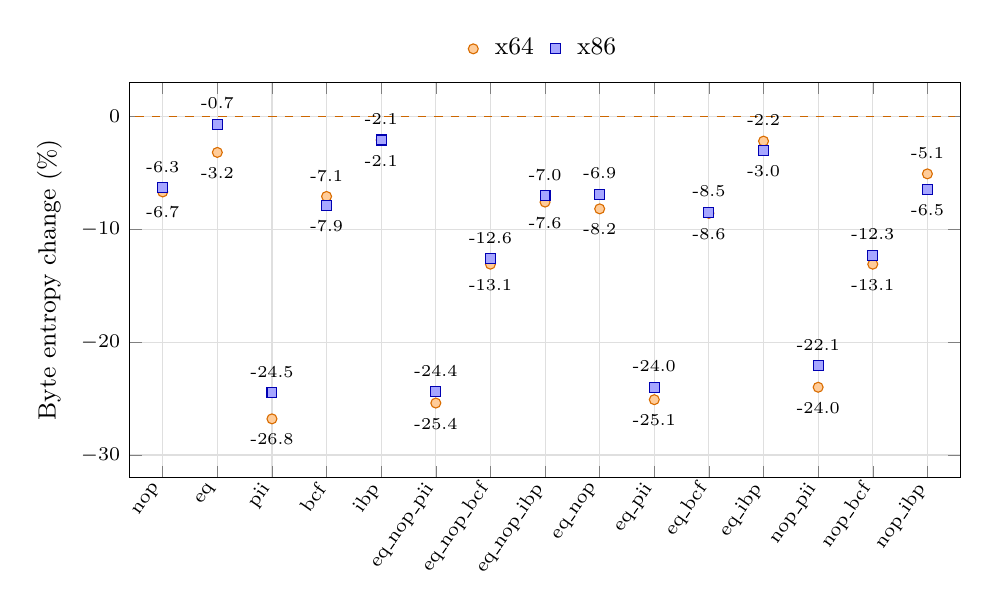
\begin{tikzpicture}
\begin{axis}[
width=\linewidth,height=6.6cm,
ylabel={Byte entropy change (\%)},ymin=-32,ymax=3,xmin=-0.6,xmax=14.6,
xtick={0,...,14},
xticklabels={nop,eq,pii,bcf,ibp,eq\_nop\_pii,eq\_nop\_bcf,eq\_nop\_ibp,eq\_nop,eq\_pii,eq\_bcf,eq\_ibp,nop\_pii,nop\_bcf,nop\_ibp},
xticklabel style={rotate=55,anchor=east,font=\scriptsize},
yticklabel style={font=\scriptsize},label style={font=\small},
grid=major,grid style={gray!25},scaled y ticks=false,
legend style={at={(0.5,1.03)},anchor=south,legend columns=2,column sep=4pt,font=\small,draw=none},
clip=false,
]
\addplot[orange!80!black,dashed,no marks,forget plot] coordinates {(-0.5,0) (14.5,0)};
\addplot[only marks,mark size=1.8pt,orange!85!black,mark=*,mark options={fill=orange!40}] coordinates {(0,-6.7) (1,-3.2) (2,-26.8) (3,-7.1) (4,-2.1) (5,-25.4) (6,-13.1) (7,-7.6) (8,-8.2) (9,-25.1) (10,-8.6) (11,-2.2) (12,-24.0) (13,-13.1) (14,-5.1)};
\addlegendentry{x64}
\node[anchor=north,yshift=-2pt,font=\fontsize{6}{7}\selectfont] at (axis cs:0,-6.7) {-6.7};
\node[anchor=north,yshift=-2pt,font=\fontsize{6}{7}\selectfont] at (axis cs:1,-3.2) {-3.2};
\node[anchor=north,yshift=-2pt,font=\fontsize{6}{7}\selectfont] at (axis cs:2,-26.8) {-26.8};
\node[anchor=south,yshift=2pt,font=\fontsize{6}{7}\selectfont] at (axis cs:3,-7.1) {-7.1};
\node[anchor=south,yshift=2pt,font=\fontsize{6}{7}\selectfont] at (axis cs:4,-2.1) {-2.1};
\node[anchor=north,yshift=-2pt,font=\fontsize{6}{7}\selectfont] at (axis cs:5,-25.4) {-25.4};
\node[anchor=north,yshift=-2pt,font=\fontsize{6}{7}\selectfont] at (axis cs:6,-13.1) {-13.1};
\node[anchor=north,yshift=-2pt,font=\fontsize{6}{7}\selectfont] at (axis cs:7,-7.6) {-7.6};
\node[anchor=north,yshift=-2pt,font=\fontsize{6}{7}\selectfont] at (axis cs:8,-8.2) {-8.2};
\node[anchor=north,yshift=-2pt,font=\fontsize{6}{7}\selectfont] at (axis cs:9,-25.1) {-25.1};
\node[anchor=north,yshift=-2pt,font=\fontsize{6}{7}\selectfont] at (axis cs:10,-8.6) {-8.6};
\node[anchor=south,yshift=2pt,font=\fontsize{6}{7}\selectfont] at (axis cs:11,-2.2) {-2.2};
\node[anchor=north,yshift=-2pt,font=\fontsize{6}{7}\selectfont] at (axis cs:12,-24.0) {-24.0};
\node[anchor=north,yshift=-2pt,font=\fontsize{6}{7}\selectfont] at (axis cs:13,-13.1) {-13.1};
\node[anchor=south,yshift=2pt,font=\fontsize{6}{7}\selectfont] at (axis cs:14,-5.1) {-5.1};
\addplot[only marks,mark size=1.8pt,blue!70!black,mark=square*,mark options={fill=blue!35}] coordinates {(0,-6.3) (1,-0.7) (2,-24.5) (3,-7.9) (4,-2.1) (5,-24.4) (6,-12.6) (7,-7.0) (8,-6.9) (9,-24.0) (10,-8.5) (11,-3.0) (12,-22.1) (13,-12.3) (14,-6.5)};
\addlegendentry{x86}
\node[anchor=south,yshift=2pt,font=\fontsize{6}{7}\selectfont] at (axis cs:0,-6.3) {-6.3};
\node[anchor=south,yshift=2pt,font=\fontsize{6}{7}\selectfont] at (axis cs:1,-0.7) {-0.7};
\node[anchor=south,yshift=2pt,font=\fontsize{6}{7}\selectfont] at (axis cs:2,-24.5) {-24.5};
\node[anchor=north,yshift=-2pt,font=\fontsize{6}{7}\selectfont] at (axis cs:3,-7.9) {-7.9};
\node[anchor=north,yshift=-2pt,font=\fontsize{6}{7}\selectfont] at (axis cs:4,-2.1) {-2.1};
\node[anchor=south,yshift=2pt,font=\fontsize{6}{7}\selectfont] at (axis cs:5,-24.4) {-24.4};
\node[anchor=south,yshift=2pt,font=\fontsize{6}{7}\selectfont] at (axis cs:6,-12.6) {-12.6};
\node[anchor=south,yshift=2pt,font=\fontsize{6}{7}\selectfont] at (axis cs:7,-7.0) {-7.0};
\node[anchor=south,yshift=2pt,font=\fontsize{6}{7}\selectfont] at (axis cs:8,-6.9) {-6.9};
\node[anchor=south,yshift=2pt,font=\fontsize{6}{7}\selectfont] at (axis cs:9,-24.0) {-24.0};
\node[anchor=south,yshift=2pt,font=\fontsize{6}{7}\selectfont] at (axis cs:10,-8.5) {-8.5};
\node[anchor=north,yshift=-2pt,font=\fontsize{6}{7}\selectfont] at (axis cs:11,-3.0) {-3.0};
\node[anchor=south,yshift=2pt,font=\fontsize{6}{7}\selectfont] at (axis cs:12,-22.1) {-22.1};
\node[anchor=south,yshift=2pt,font=\fontsize{6}{7}\selectfont] at (axis cs:13,-12.3) {-12.3};
\node[anchor=north,yshift=-2pt,font=\fontsize{6}{7}\selectfont] at (axis cs:14,-6.5) {-6.5};
\end{axis}
\end{tikzpicture}
\Description{Percentage entropy change for raw bytes; the reference level is zero. Orange circles identify x64 and blue squares identify x86.}
\caption{Percentage entropy change for raw bytes; the reference level is zero. Data from Fig.~6 of~\cite{zone_secrypt_2026}; redrawn for the present format.}
\label{fig:shan_entropy_bytes}
\end{figure}

\paragraph{Cosine Similarity.}

The frequency vectors $A$ and $B$ represent the opcode distributions of an original file and its transformed variant. Their cosine similarity is:

\[
\text{sim}(A, B) = \frac{A \cdot B}{\|A\| \, \|B\|} = \frac{\sum_{i=1}^{n} A_i B_i}{\sqrt{\sum_{i=1}^{n} A_i^2} \, \sqrt{\sum_{i=1}^{n} B_i^2}}
\]

Here $A_i$ and $B_i$ are the frequencies of opcode $i$, and $n$ is the size of their joint vocabulary. The score summarizes agreement between the two frequency profiles. Its use in assembly-obfuscation evaluation is discussed in~\cite{llmobf}; it does not establish that the programs have the same behavior.

\begin{figure}[tbp]
\centering
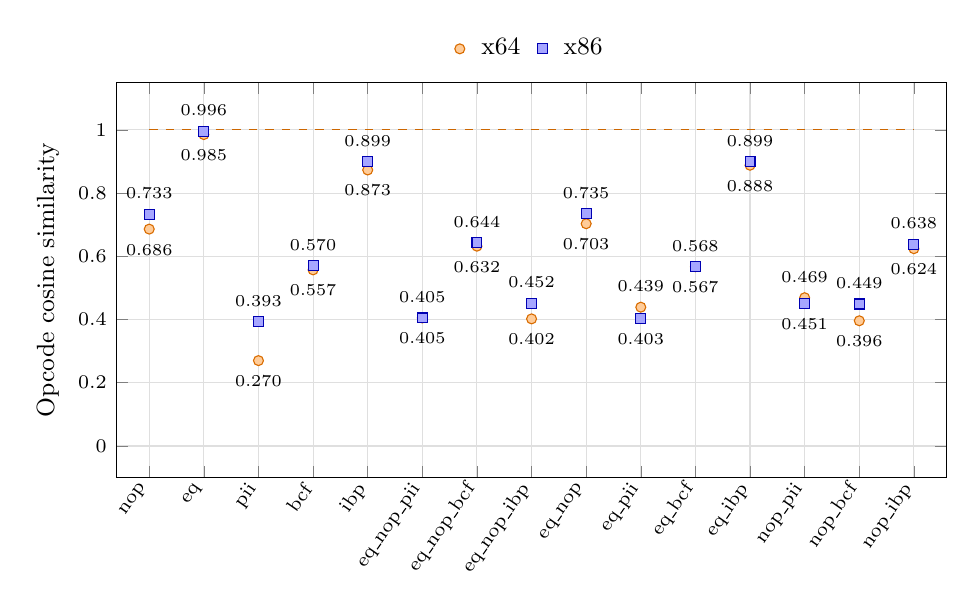
\begin{tikzpicture}
\begin{axis}[
width=\linewidth,height=6.6cm,
ylabel={Opcode cosine similarity},ymin=-0.1,ymax=1.15,xmin=-0.6,xmax=14.6,
xtick={0,...,14},
xticklabels={nop,eq,pii,bcf,ibp,eq\_nop\_pii,eq\_nop\_bcf,eq\_nop\_ibp,eq\_nop,eq\_pii,eq\_bcf,eq\_ibp,nop\_pii,nop\_bcf,nop\_ibp},
xticklabel style={rotate=55,anchor=east,font=\scriptsize},
yticklabel style={font=\scriptsize},label style={font=\small},
grid=major,grid style={gray!25},scaled y ticks=false,
legend style={at={(0.5,1.03)},anchor=south,legend columns=2,column sep=4pt,font=\small,draw=none},
clip=false,
]
\addplot[orange!80!black,dashed,no marks,forget plot] coordinates {(0,1) (14,1)};
\addplot[only marks,mark size=1.8pt,orange!85!black,mark=*,mark options={fill=orange!40}] coordinates {(0,0.686) (1,0.985) (2,0.270) (3,0.557) (4,0.873) (5,0.405) (6,0.632) (7,0.402) (8,0.703) (9,0.439) (10,0.567) (11,0.888) (12,0.469) (13,0.396) (14,0.624)};
\addlegendentry{x64}
\node[anchor=north,yshift=-2pt,font=\fontsize{6}{7}\selectfont] at (axis cs:0,0.686) {0.686};
\node[anchor=north,yshift=-2pt,font=\fontsize{6}{7}\selectfont] at (axis cs:1,0.985) {0.985};
\node[anchor=north,yshift=-2pt,font=\fontsize{6}{7}\selectfont] at (axis cs:2,0.270) {0.270};
\node[anchor=north,yshift=-2pt,font=\fontsize{6}{7}\selectfont] at (axis cs:3,0.557) {0.557};
\node[anchor=north,yshift=-2pt,font=\fontsize{6}{7}\selectfont] at (axis cs:4,0.873) {0.873};
\node[anchor=south,yshift=2pt,font=\fontsize{6}{7}\selectfont] at (axis cs:5,0.405) {0.405};
\node[anchor=north,yshift=-2pt,font=\fontsize{6}{7}\selectfont] at (axis cs:6,0.632) {0.632};
\node[anchor=north,yshift=-2pt,font=\fontsize{6}{7}\selectfont] at (axis cs:7,0.402) {0.402};
\node[anchor=north,yshift=-2pt,font=\fontsize{6}{7}\selectfont] at (axis cs:8,0.703) {0.703};
\node[anchor=south,yshift=2pt,font=\fontsize{6}{7}\selectfont] at (axis cs:9,0.439) {0.439};
\node[anchor=north,yshift=-2pt,font=\fontsize{6}{7}\selectfont] at (axis cs:10,0.567) {0.567};
\node[anchor=north,yshift=-2pt,font=\fontsize{6}{7}\selectfont] at (axis cs:11,0.888) {0.888};
\node[anchor=south,yshift=2pt,font=\fontsize{6}{7}\selectfont] at (axis cs:12,0.469) {0.469};
\node[anchor=north,yshift=-2pt,font=\fontsize{6}{7}\selectfont] at (axis cs:13,0.396) {0.396};
\node[anchor=north,yshift=-2pt,font=\fontsize{6}{7}\selectfont] at (axis cs:14,0.624) {0.624};
\addplot[only marks,mark size=1.8pt,blue!70!black,mark=square*,mark options={fill=blue!35}] coordinates {(0,0.733) (1,0.996) (2,0.393) (3,0.570) (4,0.899) (5,0.405) (6,0.644) (7,0.452) (8,0.735) (9,0.403) (10,0.568) (11,0.899) (12,0.451) (13,0.449) (14,0.638)};
\addlegendentry{x86}
\node[anchor=south,yshift=2pt,font=\fontsize{6}{7}\selectfont] at (axis cs:0,0.733) {0.733};
\node[anchor=south,yshift=2pt,font=\fontsize{6}{7}\selectfont] at (axis cs:1,0.996) {0.996};
\node[anchor=south,yshift=2pt,font=\fontsize{6}{7}\selectfont] at (axis cs:2,0.393) {0.393};
\node[anchor=south,yshift=2pt,font=\fontsize{6}{7}\selectfont] at (axis cs:3,0.570) {0.570};
\node[anchor=south,yshift=2pt,font=\fontsize{6}{7}\selectfont] at (axis cs:4,0.899) {0.899};
\node[anchor=north,yshift=-2pt,font=\fontsize{6}{7}\selectfont] at (axis cs:5,0.405) {0.405};
\node[anchor=south,yshift=2pt,font=\fontsize{6}{7}\selectfont] at (axis cs:6,0.644) {0.644};
\node[anchor=south,yshift=2pt,font=\fontsize{6}{7}\selectfont] at (axis cs:7,0.452) {0.452};
\node[anchor=south,yshift=2pt,font=\fontsize{6}{7}\selectfont] at (axis cs:8,0.735) {0.735};
\node[anchor=north,yshift=-2pt,font=\fontsize{6}{7}\selectfont] at (axis cs:9,0.403) {0.403};
\node[anchor=south,yshift=2pt,font=\fontsize{6}{7}\selectfont] at (axis cs:10,0.568) {0.568};
\node[anchor=south,yshift=2pt,font=\fontsize{6}{7}\selectfont] at (axis cs:11,0.899) {0.899};
\node[anchor=north,yshift=-2pt,font=\fontsize{6}{7}\selectfont] at (axis cs:12,0.451) {0.451};
\node[anchor=south,yshift=2pt,font=\fontsize{6}{7}\selectfont] at (axis cs:13,0.449) {0.449};
\node[anchor=south,yshift=2pt,font=\fontsize{6}{7}\selectfont] at (axis cs:14,0.638) {0.638};
\end{axis}
\end{tikzpicture}
\Description{Cosine similarity between original and transformed opcode-frequency vectors; the reference level is one. Orange circles identify x64 and blue squares identify x86.}
\caption{Cosine similarity between original and transformed opcode-frequency vectors; the reference level is one. Data from Fig.~7 of~\cite{zone_secrypt_2026}; redrawn for the present format.}
\label{fig:cosine_similarity}
\end{figure}

Instruction-frequency agreement is insufficient to validate execution: a small error can change a program's behavior while leaving that distribution almost unchanged. For this reason, the baseline used the execution checks described in Section~\ref{sec:results} to assess functionality separately.

Figure~\ref{fig:cosine_similarity} shows higher similarity for EQ and IBP than for the insertion-heavy configurations. This is consistent with their different effects on the instruction vocabulary. The larger size changes in Figure~\ref{fig:length_comparison} provide complementary information about the additional instructions; neither measurement should be substituted for a functional test.

\section{Limitations and Defensive Implications}\label{sec:limitations}
The following limitations concern the original implementation and experiments~\cite{zone_secrypt_2026}. Sections~\ref{sec:code_data}--\ref{sec:wrapping} describe subsequent work motivated by these observations; the residual limits of the added paths are discussed in Section~\ref{sec:extension_limits}.
\begin{itemize}
    \item \textbf{Instruction coverage.} Less common instructions, including the example \texttt{JRCXZ}, can require handling not exercised by this corpus. Testing a fixed collection of 102 inputs does not establish complete x86/x64 coverage.
    \item \textbf{Code--data ambiguity.} Embedded strings may partly decode as instructions. Table~\ref{tab:broken-payload} illustrates an input in which the bytes of \texttt{.exe} are interpreted as a branch. Rewriting the resulting instruction interpretation can corrupt the embedded string.
\end{itemize}

Accurate recovery of instructions and references is a broader difficulty in static binary analysis~\cite{staticdisasmTuringComplete}. General limitations of disassembly do not establish that perfect results are impossible on a bounded test corpus; they also do not excuse uncharacterized implementation failures. The reported working rates describe this implementation and these inputs.

The two examples below document the observed code--data distinction. They illustrate one failure mechanism, not a general guarantee about other payloads.

\begin{table}[t]
    \caption{Inline-data example affected by rewriting. Reproduced from Table~5 of~\cite{zone_secrypt_2026}.}
    \label{tab:broken-payload}
    \small
    \centering
    \setlength{\tabcolsep}{3pt}
    \begin{tabular}{ll}
        \hline
        \textbf{Bytes}  & \textbf{Instruction} \\ \hline
        \verb|0x109 b'\xff\xd5'|  & call  rbp \\ \hline
        \verb|0x10b b'c'|         & .byte 0x63 \\ \hline
        \verb|0x10c b'a'|         & .byte 0x61 \\ \hline
        \verb|0x10d b'l'|         & insb  byte ptr [rdi], dx \\ \hline
        \verb|0x10e b'c'|         & .byte 0x63 \\ \hline
        \verb|0x10f b'.exe'|      & js    0x178 \\ \hline
        \verb|0x113 b'\x00'|      & .byte 0x00 \\ \hline
    \end{tabular}
\end{table}

In Table~\ref{tab:broken-payload}, \texttt{calc.exe} is stored at the end of the input. Although some characters are represented as data, part of the string receives an instruction interpretation. This explains why the original implementation could modify bytes that were meant to remain data.

\begin{table}[t]
    \caption{Immediate-operand example. Reproduced from Table~6 of~\cite{zone_secrypt_2026}.}
    \label{tab:functional-payload}
    \small
    \centering
    \setlength{\tabcolsep}{3pt}
    \begin{tabular}{ll}
        \hline
        \textbf{Bytes}                  & \textbf{Instruction} \\ \hline
        \verb|0x8d b'Q'|              &  push     rcx \\ \hline
        \verb|0x8e b'H\xb9calc.exe'|  &  movabs   rcx, 0x6578652e636c6163 \\ \hline
        \verb|0x98 b'Q'|              &  push     rcx \\ \hline
        \verb|0x99 b'H\x8d\x0c\$'|     & lea      rcx, [rsp] \\ \hline
        \verb|0x9d b'H1\xd2'|          & xor      rdx, rdx \\ \hline
        \verb|0xa0 b'H\xff\xc2'|       & inc      rdx \\ \hline
        \verb|0xa3 b'H\x83\xec('|      & sub      rsp, 0x28 \\ \hline
        \verb|0xa7 b'\xff\xd0'|        & call     rax \\ \hline
    \end{tabular}
\end{table}

Table~\ref{tab:functional-payload} shows the other published example, in which the string occurs as an immediate operand at address \texttt{0x8e}. The reported transformation did not encounter the same inline-data failure. This observation is specific to that example and does not imply general immunity from rewriting errors.

\subsection{Mitigations and Countermeasures}
Changing the binary representation does not remove a program's observable actions. Defensive analysis can consider memory protections, execution patterns, API activity, and network behavior in addition to static bytes. Recognition of a transformation engine is another possibility: repeated artifacts of a common toolchain can persist across outputs, as documented for Shikata Ga Nai~\cite{sgnstrong}. Statistical or learned detectors must also account for benign programs that share similar features. These are defensive considerations arising from the study, not results of an additional detection experiment.

\section{Comparison with Shikata Ga Nai}\label{sec:comparison}

The conference paper~\cite{zone_secrypt_2026} compared Zone with the Shikata Ga Nai (SGN) polymorphic encoder~\cite{sgnarticle}. SGN combines additive-feedback encoding with a variable decoding stub. The comparison included the original x86 encoder and an unofficial x64 implementation~\cite{sgn64}; recognition of the x86 stub has been discussed in~\cite{sgnstrong}.

The published aggregate static-scan observations were:

\begin{itemize}
    \item \textbf{x64:} SGN achieved $0$\%, while Zone averaged $0.57$\% (reaching $0$\% with the PII technique).
    \item \textbf{x86:} SGN had a $10.22$\% detection rate, while Zone achieved $0.25$\% (also reaching $0$\% with PII).
\end{itemize}

The encoders also differ in the representation available after decoding. The conference paper submitted memory dumps obtained during SGN execution to VirusTotal and reported verdicts matching those for the unencoded inputs~\cite{zone_secrypt_2026}. This observation is consistent with exposure of the original representation after decoding and with prior work on extracting attack code from memory~\cite{codeExtraction}.

Zone's intended execution model retains the rewritten representation. The dump experiment nevertheless measures the recognizability of submitted memory contents; it is not a direct measurement of an endpoint product's runtime detection. Claims about deployed EDR behavior require evidence beyond this comparison.

% Added material extends the original study retained above.
\section{Code--Data Identification and Data-Preserving Rewriting}
\label{sec:code_data}
\subsection{Problem Definition}
Let an input payload be a byte sequence $B=(b_0,\ldots,b_{n-1})$.
The identification task returns candidate data intervals
$[s_j,e_j)$ in payload-relative coordinates, optionally accompanied by
a kind such as an ASCII string, a UTF-16LE string, or another data object.
A candidate identifies a proposed role for the bytes. Its acceptance
for rewriting additionally depends on the available reference evidence
and the capabilities of the data-handling layer.

The original inline-data failure in Table~\ref{tab:broken-payload}
and the immediate-operand example in Table~\ref{tab:functional-payload}
motivate this extension. Both examples and their interpretation remain
in Section~\ref{sec:limitations}; the added layer explicitly represents
candidate data and the references affected by rewriting.

The task also includes uncertainty. A region outside the recovered graph
may contain data, unobserved code, or a mixture of the two. The pipeline
retains the origin of a candidate rather than collapsing all such
regions into the same evidential category. This permits separate
assessment of candidate generation, filtering, and downstream outcomes.

\subsection{Symbolic and Heuristic Identification}
The non-LLM path combines static graph information with bounded symbolic
exploration. A CFGFast pass supplies candidate code blocks and inferred
data objects. Symbolic exploration records instruction addresses visited
under the raw-payload model. An additional graph-recovery pass can use
newly observed entries, so that dynamically observed code is not lost
merely because it was absent from the first graph.

The symbolic initial state models uninitialized registers and memory
symbolically. It does not initialize a complete Windows process or
implement all external API behavior. Exploration is bounded by a time
budget, a state/block-step limit, a pending-state limit, and solver
budgets. Reports record the stop reason and unresolved states. Reaching
a resource limit, encountering an unsupported operation, and exhausting
the current frontier have different meanings and are reported
separately.

The implementation maintains evidence at byte granularity by expanding
observed instruction starts into their decoded spans. This avoids
treating the interior bytes of an observed instruction as unexecuted
data candidates. Candidate strings are then identified with printable
ASCII and UTF-16LE patterns, including their terminators. Overlap with
observed code prevents acceptance under this string heuristic.

Static graph recovery can itself classify a string as code. For a
string that overlaps candidate graph code, the implementation requires
additional structural corroboration rather than relying on printability
alone. Other proposed regions originate from graph-inferred data or
from bytes outside recovered blocks. The latter remain uncertain and
are distinguished from stronger data candidates.

The analysis returns intervals, their kinds, and diagnostic information;
it does not prove a complete partition of the payload into code and
data. In particular, a byte not observed during this run is not thereby
proven unreachable or safe to move. The experimental assessment records
both the proposed intervals and the limits of the run that produced them.

\subsection{LLM-Based Identification}
The alternative identification path presents the input through a hex
view, a linear disassembly, and candidate printable runs. These are
different views of the same bytes. The disassembly is explicitly
heuristic, and the printable runs are candidate evidence rather than
reference labels. The model returns structured data ranges, including
offset and length, instead of a rewritten binary.

The parser checks that intervals have positive lengths, remain within
the input bounds, and do not overlap. The engine then associates
candidate ranges with its existing reference information. Ranges that
cannot be accepted by the configured pipeline are reported or rejected.
A fresh engine instance is used when applying a proposal, avoiding
reuse of partially modified state after a rejected answer.

An invalid answer can trigger another request with feedback. The
reported outcome therefore distinguishes the first proposal, later
proposals, and the final accepted result. This distinction is necessary
to attribute an observation correctly: a useful final extraction may
reflect both the model's proposal and deterministic filtering.

The number of worked examples in this classification prompt is recorded
independently of the transformation experiment. A zero-shot/two-shot
comparison of assembly transformation does not imply that the same
comparison has been performed for identification.

\subsection{Shared Data and Reference Handling}
Both identification paths connect to deterministic data-handling
routines. These routines preserve the contents selected for extraction,
track the references whose interpretation depends on the data layout,
and finalize supported references after the code layout is known.
Identification answers which regions are candidates; reference handling
determines which proposed operations are supported by the implementation.

Different architectures require different addressing treatment. The
x64 and x86 implementations therefore share a conceptual contract
without being assumed identical at operand level. A candidate accepted
in one architecture need not be accepted in the other. The evaluation
keeps architecture and reference category associated with the outcome.

The pipeline also checks output integrity, including consistency of
the preserved data contents and the supported references. These checks
can prevent an invalid output from being accepted, but they cannot
establish that all references in an arbitrary binary have been recovered.
An unsupported case is consequently distinguished from a successfully
handled case and from an output that is built but fails execution.

Analysis caching is a practical part of the implementation. Candidate
data can be reused for an input identity, while references are recomputed
against the working representation. Reproducibility requires recording
whether an identification result was computed or retrieved and the
configuration associated with the cached entry. Timing comparisons
separate these cases.

\subsection{Classification Outputs and Residual Uncertainty}
Three outputs are retained for analysis: raw candidate intervals,
intervals accepted by deterministic checks, and intervals ultimately
processed by the data layer. Equal final binaries do not establish
equal raw classifications, because filtering can remove differences.
Conversely, a correct candidate can be rejected because its reference
pattern is unsupported. That rejection is an integration limitation,
not necessarily a classification error.

The additional evaluation in Section~\ref{sec:methodology} therefore separates
classification quality from downstream functionality. Successful
execution supplies evidence about the observed behavior after data
handling, while reference annotations supply evidence about the byte
roles. Neither observation can substitute for the other.

\section{LLM-Assisted Assembly Transformation}\label{sec:llm}
\subsection{Task and Supported Transformation Families}
The transformation path asks an LLM to produce a complete modified
assembly representation for a selected family: EQ, NOP insertion, BCF,
or IBP. These families retain their meanings from the native engine;
the use of a model changes how the proposed representation is produced.
Each request selects one family so that the generated artifact and its
validation policy have an identifiable experimental condition.

PII and assembly wrapping remain native paths in the version examined
here. They are not described as LLM-generated techniques. Likewise, a
native condition combining transformations is not automatically
equivalent to several model calls in sequence. The experiment identifies
the implemented path rather than grouping all uses of the same family
under one label.

\subsection{Assembly Representation and Data Boundary}
The engine prepares an assembly representation with symbolic labels
for the relevant locations and preserves the data representation
outside the model-generated instruction text. This preparation defines
an intermediate input to the transformation task. It also determines
the reference point for several structural checks and similarity
measurements.

The model's text is assembled and associated with the data retained by
the engine. The output is therefore a product of model generation,
assembly, data handling, and validation. The experimental record retains
the identity of the original file, the intermediate representation,
and the final bytes, so that preparation-induced changes can be
distinguished from changes in the model's output.

\subsection{Zero-Shot and Two-Shot Conditions}
The initial zero-shot request contains the task specification without
worked examples. The initial two-shot request contains two examples
in addition to that specification. The example identities and prompt
versions are part of the experimental condition. Differences in their
content, not only their number, can influence the comparison.

These labels apply to the first request in a run. After rejection, a
later request may contain the previous answer and validation feedback.
Such a run remains assigned to its initial prompting condition, but its
later attempts are explicitly feedback-assisted. Reporting only the
final accepted output would hide this additional interaction.

The experimental unit is a run under a specified input, transformation,
prompt condition, and generation configuration. Repeated run numbers
are not claimed to be independently controlled model seeds unless the
service accepts and records such a parameter. Temperature, token
budget, model identifier, and service configuration are recorded
separately from the run index.

\subsection{Validation and Feedback}
Validation covers several kinds of structural evidence. Assembly must
succeed, the produced code must meet the decoding checks, tracked branch
destinations must have appropriate boundaries, and the expected data
representation must remain consistent. Additional checks depend on the
selected family and examine whether the output still contains the
required instruction structure or applies a nontrivial transformation.

These checks are deliberately narrower than semantic equivalence.
An output can pass structural validation yet behave differently; a
conservative check can also reject an output that would have performed
the expected behavior. The assessment records the reason for each
rejection rather than treating all rejected answers as one category.

For supported test cases, a functional verifier can participate in the
generation loop. If that verifier is also used to select accepted
outputs, a later test based on the same observable is conditional on
selection. The article distinguishes this pipeline acceptance criterion
from an independent functional assessment and reports attempts that
exhaust the allowed budget.

\subsection{What Is Attributed to the Model}
Three aspects are considered separately: whether an answer can be
assembled, whether the complete pipeline accepts it, and whether an
accepted output satisfies the reported functional check. Deterministic
preparation and validation are part of the system contribution rather
than capabilities attributed to the model alone.

The run record includes elapsed time, API usage when supplied by the
service, rejected attempts, and the accepted artifact. Estimated cost
is derived from the stated tariff snapshot; it is not presented as an
invoice. Resumed jobs and reused outputs are identified so that they
are not counted as additional generation calls.

\section{Integration of Assembly Wrapping}\label{sec:wrapping}
\subsection{Existing Technique and Contribution}
Assembly wrapping is an established technique based on alternative
instruction interpretations~\cite{assembly_wrapping}. Its inclusion in
this article does not claim invention of the underlying idea. The
extension contributes an implementation in Zone, interaction with the
engine's instruction and data representations, and a separate empirical
assessment.

The relevant conceptual property is that the instruction interpretation
obtained by a particular static decoding need not be the instruction
stream followed during execution. This property makes it especially
important to identify which representation is used by a similarity or
coverage measurement. A statistic from the static view and one from
the intended execution view answer different questions.

\subsection{Integration and Supported Inputs}
Wrapping is integrated with the native rewriting infrastructure and
depends on an instruction representation adequate for the selected
input. It must also interact with the final data layout and the
references affected by changes in instruction placement. Construction
can be refused when the required input interpretation is incomplete
or an unsupported case is encountered.

Some instructions or local regions are handled differently from the
main wrapped representation. The assessment therefore records the
proportion represented by wrapping, retained regions, output size,
construction failures, and functional outcomes. A claim about the
whole output must not be inferred solely from the fraction of
instructions accepted by one internal stage.

The experiment distinguishes wrapping alone, the chosen combined
native condition, and the corresponding preparation-only controls.
Their names identify complete configurations, including data handling
and architecture. Implementation availability and successful build
are reported separately from empirical functionality.

\subsection{x86 Port and Development Status}
The x64 implementation is available for assessment. The x86 port is
under active development at the time of this draft. Register width,
instruction encodings, and addressing assumptions require
architecture-specific treatment, so an x64 outcome is not transferred
to the x86 column of a result table.

The result layout reserves separate x86 entries. Those entries remain
marked as development work until a frozen version and its assessment
are available. If the port changes during a campaign, its new results
are associated with the new version; they are not silently appended
to results from an earlier implementation.

\subsection{Assessment Boundary}
Wrapping is assessed with the same separation of construction,
functionality, and representation measurements used for other methods.
In particular, a failure to construct an output remains part of the
overall outcome. Reporting functionality only for constructed binaries
can describe accepted artifacts but does not describe availability
across all attempted cases. Section~\ref{sec:methodology} defines both
denominators.

\section{Additional Experimental Methodology}\label{sec:methodology}
\subsection{Questions and Experimental Record}
The additional experiments complement the original fifteen-configuration
study. They examine (i) identification quality and agreement between
the two code--data paths, (ii) construction and functional outcomes
after data handling, (iii) architecture-specific wrapping outcomes,
and (iv) zero-shot versus two-shot LLM transformation. The original
corpus and its measurements remain those of
Sections~\ref{sec:results} and~\ref{sect:var_metrics}.

Each new campaign records distinct inputs, selection criteria,
architecture, configuration, repetitions, input/output hashes, and
engine version or snapshot. A subset selected for low historical
working rate is reported as a subset, not a new assessment of the
whole corpus. Model identifier, prompt examples, generation parameters,
retry policy, dependency versions, and cache status are retained where
applicable. A run is distinguished from attempts within that run and
from a reused artifact; run numbers do not imply controlled model seeds.

\subsection{Code--Data Quality and Downstream Outcomes}
Reference-based identification measures use independently annotated
data-byte offsets $G$ and predicted offsets $P$. With data as the
positive class, precision is $|P\cap G|/|P|$, recall is
$|P\cap G|/|G|$, and $F_1$ is their harmonic mean. Undefined cases and
unresolved reference bytes are identified explicitly. Interval-level
agreement complements byte scores, with the boundary or overlap rule
specified in the report. Raw candidates and accepted intervals are
assessed separately to distinguish classification from filtering.

Without independent annotations, the analysis is a case study of
agreement and downstream functionality. Agreement with the symbolic
method does not make that method ground truth, and byte-identical
outputs do not establish identical raw proposals. Analysis limits,
unresolved states, and computed versus cached runtimes accompany the
identification outcomes.

For $N$ planned cases, $B$ accepted binaries, and $W$ successful
functional checks, the additional assessment reports
\begin{equation}
\mathrm{BuildRate}=B/N,\qquad
\mathrm{WorkingRate}_{\mathrm{all}}=W/N,\qquad
\mathrm{WorkingRate}_{\mathrm{built}}=W/B.
\end{equation}
Counts accompany percentages. Unbuilt cases remain in the planned-case
denominator, and uncompleted tests remain distinct from completed
failures. The observable, harness version, architecture, and observation
window are stated. Connections, open ports, dialogs, and clean
termination provide different empirical checks rather than a general
proof of equivalence.

For LLM runs, initial acceptance and acceptance within the retry budget
are separated. If the functional verifier participates in output
selection, the pass rate on accepted outputs is conditional on that
selection. Exhausted and restarted runs, including their time and
cost, remain part of the record.

\subsection{Static Verdicts, Similarity, and Cost}
The published detection definition is retained for comparison. For a
completed file, $d_i=m_i/a_i$ is the malicious-verdict fraction, with
$m_i$ malicious verdicts and $a_i$ engines under the declared eligibility
rule. The new report also distinguishes the fraction of completed
files with any malicious verdict:
\begin{equation}
\overline d=\frac{1}{F}\sum_{i=1}^{F}d_i,\qquad
q=\frac{1}{F}\sum_{i=1}^{F}\mathbf{1}[m_i>0].
\end{equation}
Unsupported engines, errors, timeouts, scan dates, and pending analyses
are accounted for explicitly. Pending is not zero detection. Identical
hashes may reuse a scan while retaining their membership in several
experimental conditions. The aggregation states whether payloads,
runs, or distinct binaries receive equal weight.

The original size, entropy, and cosine measurements are retained in
Section~\ref{sect:var_metrics}. The additional LLM validation score uses
\texttt{SequenceMatcher} on normalized instruction signatures,
not cosine similarity~\cite{python_difflib}. Its matching-block ratio
is $2M/(u+v)$ for $M$ matched elements and sequence lengths $u,v$.
The NOP condition additionally removes recognized no-op operations;
a score of one under that representation does not imply byte identity.
The original file and the prepared intermediate representation are
distinguished as comparison references. Any new cosine measure states
its token vocabulary and whether comparisons are paired or pooled.
Wrapping measurements also identify the decoding view.

Distinct output hashes characterize exact diversity independently of
similarity. Size is reported as bytes and paired relative change.
Timing separates analysis, preparation, API calls, and local checks
where available. Costs include rejected attempts and state the tariff
snapshot and estimation rule. Repetitions of the same payload are
grouped for uncertainty analysis; small pilots retain case-level scope.

\subsection{Validity of the Extensions}\label{sec:extension_limits}
The original limitations remain relevant. Bounded exploration can
miss paths because of missing environment behavior or resource limits;
LLM and deterministic paths can share errors; and structural validation
does not establish full semantic preservation. Changes in the harness,
dependencies, input selection, or engine version can affect apparent
working-rate improvements. Historical and new scans also differ in
time and service conditions. Architecture-specific development,
especially x86 wrapping, is associated with its own frozen version
and assessment rather than inferred from x64 results.
\draftnote{Finalize input counts, repetitions, model configuration,
annotations, harness, scan eligibility, and aggregation from the completed
campaigns. Preserve the original measurements as the published comparison.}

\section{Additional Experimental Results}\label{sec:extended_results}
The results below are additional to the full published study retained
in Sections~\ref{sec:results}--\ref{sec:comparison}. New campaign outcomes
will be associated with their own inputs, versions, and observation
protocol. They do not silently replace the historical measurements.

\subsection{Code--Data Identification and Functional Outcomes}
\draftnote{Insert the completed comparison, independent reference
annotations if available, candidate/accepted interval results, analysis
time, and functional outcomes after extraction. Keep selection and
architecture explicit.}
\begin{table}[t]
\caption{Additional code--data assessment; entries await finalized
experiments. Use agreement/case-study reporting if independent labels
are unavailable.}
\label{tab:new_data_results}
\centering\small
\begin{tabularx}{\linewidth}{@{}Yllll@{}}
\toprule
Method & Inputs & Precision$_D$ & Recall$_D$ & $F_{1,D}$ \\
\midrule
Symbolic/heuristic & \pending & \pending & \pending & \pending \\
LLM classification & \pending & \pending & \pending & \pending \\
\bottomrule
\end{tabularx}
\end{table}
The final analysis will separate a changed classification from a
changed acceptance decision or functional oracle. Any current
working-rate comparison with the original study will state changes
in corpus selection, preparation, and testing conditions.

\subsection{Assembly Wrapping}
\draftnote{Insert build counts, working rates, size, diversity, and
completed static scans. x86 remains development work until its version
and architecture-specific campaign are fixed.}
\begin{table}[t]
\caption{Additional wrapping outcomes. Report both planned-case and
constructed-output working rates; static results refer to completed scans.}
\label{tab:new_wrap_results}
\centering\small
\begin{tabularx}{\linewidth}{@{}Yllll@{}}
\toprule
Condition & $B/N$ & $W/N$ & $W/B$ & $\overline d$ \\
\midrule
x64 wrapping & \pending & \pending & \pending & \pending \\
x64 wrapping, combined & \pending & \pending & \pending & \pending \\
x86 wrapping & \multicolumn{4}{c}{\dev} \\
x86 wrapping, combined & \multicolumn{4}{c}{\dev} \\
\bottomrule
\end{tabularx}
\end{table}

\subsection{LLM Transformation: Zero-Shot versus Two-Shot}
\draftnote{Insert the final input/run counts, initial and final acceptance,
functional outcomes, static verdicts, normalized sequence similarity,
output uniqueness, attempts, time, and estimated cost. Record the scope
of the pilot and the role of the generation-time verifier.}
\begin{table}[t]
\caption{Additional LLM transformation results. Similarity denotes
the normalized sequence score, distinct from the historical cosine
measure. Pending scans have no measured detection fraction.}
\label{tab:new_llm_results}
\centering\small
\begin{tabularx}{\linewidth}{@{}Yllll@{}}
\toprule
Family / shots & Runs & $W/N$ & $\overline d$ & Similarity \\
\midrule
EQ / 0 & \pending & \pending & \pending & \pending \\
EQ / 2 & \pending & \pending & \pending & \pending \\
NOP / 0 & \pending & \pending & \pending & \pending \\
NOP / 2 & \pending & \pending & \pending & \pending \\
BCF / 0 & \pending & \pending & \pending & \pending \\
BCF / 2 & \pending & \pending & \pending & \pending \\
IBP / 0 & \pending & \pending & \pending & \pending \\
IBP / 2 & \pending & \pending & \pending & \pending \\
\bottomrule
\end{tabularx}
\end{table}
The comparison will interpret representation changes alongside
construction and functional outcomes. Similarity alone does not
establish correctness, and accepted outputs do not characterize the
success rate of first attempts or exhausted runs.


\section{Related Work}\label{sect:related_work}
Instruction-level obfuscation has been studied in both offensive and defensive settings~\cite{survey1,survey2}. Earlier engines, including W95/Regswap~\cite{desai2010highly} and MetaPHOR~\cite{MetaPHOR}, explored register substitution and code reorganization. Instruction substitution, insertion, and control-flow transformations underpin the techniques summarized here~\cite{desai2008towards,desai2010highly,szor2001hunting,bin2binobf,llvmobf}.

Polymorphic encoding provides a related but distinct representation strategy. Analyses of SGN describe both the variation in its decoding stub and opportunities to recognize it~\cite{sgn64,sgnstrong}; memory-extraction research addresses the body recovered during execution~\cite{codeExtraction}. For metamorphic programs, detection studies have considered Hidden Markov Models~\cite{wong2006hunting,desai2010highly}, API-trace similarity~\cite{identifyingmeth}, and genetic-algorithm-based methods~\cite{methgenetic}.

More recent work examines LLM-based assembly transformation, including the MetamorphASM benchmark and its MAD dataset~\cite{llmobf,llm2}. Compiler-based systems such as Obfuscator-LLVM~\cite{llvmobf} offer another setting, with access to source-level or intermediate information during compilation.

The contribution of the conference paper was its payload-level \emph{bin2bin} study, the PII design, and the joint evaluation of selected transformation configurations~\cite{zone_secrypt_2026}. Those contributions are the starting point of this manuscript, rather than new claims of the extended version.


The extensions additionally connect data identification with bounded
symbolic and static analysis~\cite{angr_cfg_docs}, and distinguish LLM
classification from assembly transformation. Assembly wrapping is
attributed to its existing description and acknowledged antecedents
in overlapping instructions~\cite{assembly_wrapping}; its integration
into Zone is assessed as an implementation contribution. These new
directions build on the earlier payload-level study while preserving
its detailed results for comparison.

\section{Conclusions}\label{sec:conclusion3}
Zone provides a binary-to-binary setting for studying metamorphic
transformation of compact Windows payloads. The original study of
102 inputs and fifteen configurations remains the empirical foundation
of this extended article. Its detection, functionality, size, entropy,
and similarity results expose different effects of rewriting:
lower raw-file malicious-verdict fractions coexist with substantial
variation in functional outcomes and representation overhead.
The PII design and the SGN comparison are retained within the scope
of those published experiments.

The extension develops the code--data limitation identified by that
study into an explicit identification and data-handling layer.
Symbolic and heuristic analysis and an LLM-based alternative feed
deterministic handling of accepted candidates. A separate LLM path
supports assembly transformation with zero-shot and two-shot
conditions, validation, and feedback. Integration of assembly wrapping
adds an existing technique to the engine; its x86 port remains under
development pending architecture-specific assessment.

The additional protocol separates classification quality, construction,
working rate, static verdicts, similarity, diversity, and cost. These
measurements extend rather than replace the original evaluation.
Their interpretation remains tied to the tested inputs, analysis
limits, functional observables, and scan conditions. Complete semantic
equivalence and general endpoint behavior require evidence beyond
those observations.
\draftnote{Add the principal completed extension findings here and in
the abstract. Keep the original findings and update the x86 status only
after its campaign is finalized.}

\begin{credits}
\subsubsection{\ackname}
This work was partially funded by the University of Perugia's project ``Fighting Cybercrime with OSINT'' (FICO), Civil Safety and Security for Society (WP2).

\subsubsection{\discintname}
\emph{To be completed by the authors before submission.}
% TODO-AUTHORS: Insert the truthful competing-interests declaration. Do not
% replace this with a no-conflict declaration until every author has confirmed it.
\end{credits}

\bibliographystyle{splncs04}
\bibliography{bibliography}
\end{document}


